% =============================================================================
% Real-Time RFID Employee Attendance System — Project Report
% Compile with: xelatex document.tex && biber document && xelatex document.tex && xelatex document.tex
% =============================================================================
\documentclass[12pt, a4paper]{report}

% ---------------------------------------------------------------------------
% Fonts — Times New Roman body text at 12pt, via XeLaTeX + fontspec
% ---------------------------------------------------------------------------
\usepackage{fontspec}
\setmainfont{Times New Roman}
\newfontfamily\courierfont{Courier New}

% ---------------------------------------------------------------------------
% Page geometry
% ---------------------------------------------------------------------------
\usepackage[a4paper, left=1.5in, right=1in, top=1in, bottom=1in]{geometry}
\usepackage{setspace}
\onehalfspacing

% ---------------------------------------------------------------------------
% Core packages
% ---------------------------------------------------------------------------
\usepackage{graphicx}
\usepackage[justification=centering]{caption}
\usepackage{subcaption}
\graphicspath{{pictures/}{pictures/generated/}}

\usepackage{amsmath}
\usepackage{array}
\usepackage{booktabs}
\usepackage{longtable}
\usepackage{multirow}
\usepackage{tabularx}
\usepackage{float}
\usepackage{enumitem}
\usepackage{xcolor}
\usepackage{tikz}
\usetikzlibrary{shapes.geometric, arrows.meta, positioning, fit, calc, backgrounds}
\usepackage{pgfgantt}
\usepackage{listings}
\usepackage{hyperref}
\usepackage[a-1b]{pdfx}[2020/01/14]
\usepackage{fancyhdr}
\usepackage{titlesec}
\usepackage[skip=10pt]{parskip}
\usepackage{csquotes}

% ---------------------------------------------------------------------------
% Bibliography — Harvard (author-year) style via biblatex/biber
% ---------------------------------------------------------------------------
\usepackage[
    backend=biber,
    style=authoryear,
    dashed=false,
    maxcitenames=2,
    maxbibnames=99,
    sorting=nyt,
    natbib=true
]{biblatex}
\addbibresource{references.bib}
\DeclareNameAlias{sortname}{family-given}

% ---------------------------------------------------------------------------
% Hyperref setup
% ---------------------------------------------------------------------------
\hypersetup{
    colorlinks=true,
    linkcolor=black,
    citecolor=black,
    urlcolor=blue,
    bookmarksnumbered=true,
    pdfstartview=FitH
}

% ---------------------------------------------------------------------------
% Code listings (used in Chapter 3 snippets and Appendix A firmware source)
% ---------------------------------------------------------------------------
\lstdefinestyle{codebase}{
    basicstyle=\courierfont\scriptsize,
    keywordstyle=\color{blue!70!black}\bfseries,
    commentstyle=\color{green!40!black}\itshape,
    stringstyle=\color{orange!70!black},
    numbers=left,
    numberstyle=\tiny\color{gray},
    numbersep=5pt,
    frame=single,
    breaklines=true,
    breakatwhitespace=false,
    breakindent=0pt,
    showstringspaces=false,
    tabsize=2,
    columns=fullflexible,
    keepspaces=true,
    xleftmargin=1.3em,
    linewidth=\dimexpr\linewidth-1.3em\relax
}
\lstset{style=codebase}

% ---------------------------------------------------------------------------
% Chapter / section heading style
% ---------------------------------------------------------------------------
\titleformat{\chapter}[display]
    {\normalfont\bfseries\LARGE}{\chaptertitlename\ \thechapter}{10pt}{\Huge}
\titlespacing*{\chapter}{0pt}{-20pt}{20pt}

\setlength{\headheight}{15pt}
\pagestyle{fancy}
\fancyhf{}
\fancyhead[R]{\thepage}
\fancyhead[L]{\nouppercase{\leftmark}}
\renewcommand{\headrulewidth}{0.4pt}

% ---------------------------------------------------------------------------
% Custom commands
% ---------------------------------------------------------------------------
\newcommand{\systemname}{Real-Time RFID Employee Attendance System}

\begin{document}

% =============================================================================
% FRONT MATTER
% =============================================================================
\pagenumbering{roman}

\begin{titlepage}
    \centering
    \vspace*{0.3cm}

    
\includegraphics[width=0.42\textwidth]{telone_logo.png}\\[0.6cm]

    {\large\bfseries TELONE CENTRE FOR LEARNING}\\[0.2cm]
    {\normalsize Department of Telecommunications Engineering}\\[1.4cm]

    \rule{\linewidth}{0.6pt}\\[0.4cm]
    {\LARGE\bfseries Enhancing Workforce Management at Infor Relay Systems (Pvt) Ltd Through Implementation of a Real-Time RFID Employee Attendance System}\\[0.4cm]
    \rule{\linewidth}{0.6pt}\\[1.4cm]

    {\normalsize A project report submitted in partial fulfilment of the requirements for the\\
    National Diploma in Telecommunications Engineering\\[0.2cm]
    \textit{\footnotesize (Qualification level to be confirmed against the student's official programme handbook)}}\\[1.6cm]

    \begin{tabular}{rl}
        \textbf{Student Name:} & Dennis Kunakah \\[4pt]
        \textbf{Registration Number:} & T2329469T \\[4pt]
        \textbf{Programme:} & Telecommunications Engineering \\[4pt]
        \textbf{Host Organisation:} & Infor Relay Systems (Pvt) Ltd \\[4pt]
        \textbf{Supervisor:} & \textit{[Supervisor's Name]} \\[4pt]
    \end{tabular}\\[1.8cm]

    {\normalsize August 2026}

    \vfill
\end{titlepage}

\chapter*{Declaration}
\addcontentsline{toc}{chapter}{Declaration}

I, Dennis Kunakah, declare that this project report is my own original work, carried out during my industrial attachment at Infor Relay Systems (Pvt) Ltd, and that it has not been submitted before for any other qualification. Where I have drawn on the work of others, this has been fully acknowledged through in-text citation and referencing.

\vspace{2.5cm}
\noindent
\begin{tabular}{@{}ll}
    Signature: & \makebox[6cm]{\hrulefill} \\[4pt]
    Date: & \makebox[6cm]{\hrulefill} \\
\end{tabular}

\vspace{2cm}
\noindent\textit{Supervisor's approval}

\vspace{1cm}
\noindent
\begin{tabular}{@{}ll}
    Signature: & \makebox[6cm]{\hrulefill} \\[4pt]
    Date: & \makebox[6cm]{\hrulefill} \\
\end{tabular}

\clearpage

\chapter*{Acknowledgements}
\addcontentsline{toc}{chapter}{Acknowledgements}

I would like to thank the management and staff of Infor Relay Systems (Pvt) Ltd for hosting my industrial attachment and for giving me the opportunity to identify a real workplace problem and build a working solution for it. Particular thanks go to my workplace supervisor and colleagues in the technical department, who supported the installation and testing of the attendance system on-site.

I am also grateful to my supervisor and the lecturers at TelOne Centre for Learning, whose guidance shaped both the technical direction of this project and the way it is presented in this report. Finally, I thank my family and friends for their patience and encouragement throughout the attachment period.

\clearpage


\tableofcontents
\clearpage
\listoffigures
\clearpage
\listoftables
\clearpage

% =============================================================================
% MAIN MATTER
% =============================================================================
\pagenumbering{arabic}

\chapter{Introduction}
\label{ch:introduction}

\section{Abstract}

Infor Relay Systems (Pvt) Ltd, like many organisations, has relied on a paper attendance register and supervisor sign-off to track when employees arrive and leave work. This method sounds simple, but in practice it creates more problems than it solves. Registers get filled in late, entries go missing, and it is genuinely hard to prove exactly when someone clocked in on a busy morning. Those small gaps add up: payroll staff spend hours reconciling hand-written times, and the business loses confidence in the numbers it is paying people against.

This project set out to replace that register with something that records the moment automatically. The result is a Real-Time RFID Employee Attendance System built around an ESP32 microcontroller, an MFRC522 RFID reader, and a purpose-built Next.js web application running on a PC at the front desk. Each employee is issued an RFID card. Tapping it at the reader on the way in and again on the way out is all that is required — the station beeps, the LCD confirms the name, and the PC dashboard updates within seconds to show who is \textit{Present}, who has \textit{Left}, and who is \textit{Absent} for the day.

What makes the design worth documenting is not the RFID reader itself — that part is well understood — but the fact that the reader station keeps working when the network does not. Every tap is written to the device's own flash storage first; forwarding it live to the server is a bonus, not a requirement. If Wi-Fi drops or the PC is rebooted, taps queue locally and drain automatically once the connection returns. Two indicator LEDs make the difference between "no Wi-Fi" and "Wi-Fi is fine but the server is down" visible to whoever is on the door, instead of leaving them guessing. This report walks through why that design was chosen, how it was built and wired, what it looks like running, and how well it met the objectives set out at the start of the attachment.

\section{Background of the Study}

Attendance tracking sits at the intersection of two things every organisation cares about: paying people correctly and knowing who is on site. At Infor Relay Systems (Pvt) Ltd, both of those depend on a manual register signed at a supervisor's desk. It is a method that has worked, in a loose sense, for a long time — but it was never built to survive a busy shift change, a supervisor who is away, or a payroll clerk who has to turn scrawled timestamps into billable hours by the end of the month.

The wider literature backs up what the company was already experiencing informally. Manual and shared-login systems are consistently identified as the easiest to abuse, because they have no built-in way to verify that the person recorded is the person who actually showed up \parencite{oloid2025buddy}. The practice of one employee marking attendance for another — commonly called buddy punching — is a well-documented consequence of exactly this kind of system, and it directly inflates the hours a company believes it owes in wages \parencite{qandle2025buddy}. RFID-based attendance has become one of the more common responses to this problem across both educational and industrial settings, precisely because a card is quick to tap, hard to forge casually, and ties a specific identifier to a specific timestamp \parencite{want2006introduction, landt2005history}.

A number of recent student projects have applied the same core idea — an ESP32 paired with an MFRC522 reader — to build low-cost, real-time attendance systems for schools and small offices \parencite{singh2022iot, yadav2025rfid, hutabarat2025implementation}. These projects consistently report faster, more reliable attendance capture than manual alternatives, though most of them assume the device is always online and log straight to a spreadsheet or a single database call. That assumption does not hold well in a factory or workshop environment, where Wi-Fi coverage at a shop-floor entrance is often patchy. The design adopted in this project borrows the RFID-plus-microcontroller approach from that body of work, but treats network connectivity as something that can fail, not something to assume.

\section{Problem Statement}

At Infor Relay Systems (Pvt) Ltd, recording attendance on time and correctly is very important for smooth operations and good service delivery. However, many employees record their attendance late, and the paper register offers no real safeguard against a colleague signing in on someone else's behalf. This causes problems such as incorrect attendance records, payroll errors, poor planning, and reduced productivity. Errors introduced at the point of capture are expensive to fix later: a payroll clerk cannot always tell, weeks after the fact, whether a blank entry means an employee was absent or simply forgot to sign the book. There is, therefore, a clear need to improve the attendance recording process to make it faster, more accurate, and harder to manipulate, without asking staff to learn a complicated new system.

\section{Aim}

To develop a reliable and efficient RFID employee attendance system that enhances the accuracy of attendance tracking and reduces errors in the payroll process.

\section{Objectives}

\begin{enumerate}[label=\arabic*.]
    \item To automate attendance tracking, so that arrival and departure times are captured the instant an employee taps their card, without manual data entry.
    \item To ensure accurate labour costing, by producing attendance records precise and trustworthy enough to support payroll calculation.
    \item To integrate RFID attendance with existing systems, so that the data captured at the reader is usable by the processes that already run the business.
\end{enumerate}

\section{Proposed Solution}

The proposed solution is a two-part system: an ESP32-based reader station at the entrance, and a Next.js web application running on a PC that acts as the single source of truth for every student or employee record and every attendance event. Each person taps an RFID card once on arrival and once on departure. The dashboard derives three states from those two taps — \textit{Present} (arrived, not yet left), \textit{Left} (arrived and departed), and \textit{Absent} (no tap at all) — rather than storing a status field directly, which keeps the underlying data model small and avoids records ever going stale or contradicting the timestamps they are built from.

The reader station is deliberately designed to be useful even when the network is not. It always writes a tap to its own local flash storage before attempting to forward it, so a queue of pending taps survives a power cycle and drains automatically the moment the server becomes reachable again. The station resolves the server's address using mDNS rather than a fixed IP address, which means the front-desk PC can be restarted, or the router can hand out a new address, without anyone needing to reflash the device. Two separate status LEDs — one for Wi-Fi, one for the application server — let front-desk staff immediately tell "no network" apart from "network is fine, but the app is down," which a single combined status light cannot do. Unknown cards are never silently ignored or auto-registered: a tap from an unrecognised UID is logged and surfaced on the dashboard as an alert with a one-click \textit{Register} action, so a new employee's card becomes usable within seconds of an administrator confirming it. Chapter 3 sets out the full technology stack, wiring, and software architecture behind this design in detail.

\section{Justification of the Study}

Manual attendance and shared verification processes are a documented source of payroll inaccuracy and time theft, not just an operational inconvenience \parencite{qandle2025buddy, oloid2025buddy}. Automating capture at the point of arrival closes that gap directly: RFID technology guarantees that the record created belongs to the card that was tapped, and removes the opportunity for a colleague to sign in on someone else's behalf \parencite{shukla2019conceptual}. For Infor Relay Systems (Pvt) Ltd specifically, a faster and more trustworthy attendance record shortens the time payroll staff spend reconciling hours, reduces disputes over pay, and gives management an accurate, real-time view of who is on site — all without requiring a change to how employees already move through the entrance each day.

\section{Scope and Limitations}

The system covers card-based arrival and departure logging for a single entrance, student/employee registration, event management (so attendance can be scoped to a shift, orientation day, or other defined period), and a dashboard showing live Present/Left/Absent status. It does not, in its current form, perform biometric verification, so it cannot fully rule out one employee tapping in for another if a card is shared voluntarily — a limitation shared with every RFID-only system and discussed further as an area for future work in Chapter 5. It also does not yet push attendance data directly into a payroll or HR system; that integration is addressed as a partially achieved objective in Chapter 4. The project was built and demonstrated on a single reader station during the attachment period; scaling to multiple entrances is a straightforward extension of the same architecture but was outside the time available for this attachment.

\section{Structure of the Report}

The remainder of this report is organised as follows. Chapter 2 reviews existing literature on RFID-based attendance systems, the trade-offs between RFID and biometric approaches, and offline-first design for embedded devices. Chapter 3 describes the methodology: the system architecture, hardware selection and wiring, the custom PCB, the software stack, and the bill of quantities for the components purchased. Chapter 4 presents the results, evaluating the finished system against each objective set out above. Chapter 5 concludes the report and gives recommendations for future work, along with the project timeline.

\chapter{Literature Review}
\label{ch:litreview}

\section{Introduction}

This chapter reviews the technology and prior work that shaped the design decisions behind the attendance system. It starts with the fundamentals of RFID, moves through attendance systems that other students and researchers have already built with similar hardware, and then looks specifically at the two design choices that set this project apart from a typical class project: treating the network as unreliable by default, and separating "no Wi-Fi" from "Wi-Fi fine, server down" as two distinct failure states. The chapter closes by identifying the gap in the existing work that this project tries to fill.

\section{Fundamentals of RFID Technology}

Radio Frequency Identification (RFID) is not a new idea. \textcite{landt2005history} traces its roots back to radar research in the 1940s, long before anyone thought to attach a chip to a plastic card. What matters for this project is the more recent, practical form of the technology: a small passive tag containing an antenna and a chip, which draws its power from the electromagnetic field generated by a nearby reader and responds with a unique identifier. \textcite{want2006introduction} describes this exchange clearly — the tag needs no battery of its own, which is exactly why RFID cards can sit in a wallet for years and still work the first time they are tapped. \textcite{finkenzeller2010rfid} goes further into the physics and standards involved, and is a useful reference for anyone who needs to understand why a 13.56 MHz reader such as the MFRC522 used in this project reads a card reliably from a few centimetres away but not from across a room — the read range is a direct consequence of how the tag is powered, not a limitation that can be tuned away in software.

For an attendance system, the property that matters most is that the tag's identifier is fixed and unique. A card cannot be "typed in" wrong, and unlike a signature or a manually entered employee number, it does not depend on the person at the desk transcribing anything correctly. That single property is the foundation the rest of this project's design rests on.

\section{RFID-Based Attendance Systems: Related Work}

RFID attendance systems built around low-cost microcontrollers are now common enough in student and small-scale projects that a reasonably clear pattern has emerged. \textcite{singh2022iot} built an IoT-based digital attendance system using an ESP32 and an RFID reader, logging taps to a live database and reporting that it reduced the manual effort involved in daily attendance capture considerably compared to a paper register. \textcite{yadav2025rfid} took a lighter-weight approach, using an ESP32 and RC522 reader to log attendance directly into a Google Sheet, which keeps the system cheap to deploy but ties every tap to an active internet connection at the moment it happens. \textcite{hutabarat2025implementation} combined the same ESP32-plus-RC522 pairing with a MySQL database and a PHP web interface for a university campus, and specifically credits the system with reducing proxy attendance — a version of the same buddy-punching problem this project is trying to solve for a workplace rather than a classroom. \textcite{turpo2025edurfid} pushed the cost angle furthest, reporting a 94\% cost reduction compared to commercial RFID attendance products by building on a Raspberry Pi and Arduino combination for rural schools in Peru, with a claimed sub-second response time per tap.

Looking across this body of work as a whole, \textcite{ishaq2023iot} carried out a systematic literature review of IoT-based RFID attendance systems and found that most published implementations follow the same broad shape: a microcontroller, an RFID reader, and a live connection to a server or spreadsheet. Very few of the systems reviewed treated connectivity loss as something the design needed to plan for, rather than an edge case to be ignored. That observation lines up with what this project encountered directly during the attachment: a factory entrance is not a lecture hall with dependable Wi-Fi, and a system that only works while the network is up is not good enough for a real workplace.

On the payroll side specifically, \textcite{shukla2019conceptual} proposed a conceptual framework for combining RFID with biometric verification to improve both payroll accuracy and attendance monitoring, arguing that the two technologies address different weaknesses — RFID is fast and cheap, biometrics closes the "borrowed card" gap that RFID alone cannot. That framework is a useful reference point for this project's own limitations, discussed later in Chapter 5, since the system built here uses RFID alone and therefore inherits the same borrowed-card weakness that Shukla and Bhandari set out to solve.

\section{RFID Versus Biometric and Other Identification Methods}

RFID is not the only option for automated attendance capture, and it is worth being honest about where it is weaker than the alternatives. Biometric methods — fingerprint or facial recognition — identify the person directly rather than an object the person is carrying, which closes the door on one employee tapping in for another \parencite{nialabs2025biometric}. \textcite{peniel2025rfid} frames the choice as a trade-off rather than a simple case of one technology being better: RFID is faster per transaction, tolerant of dirty or gloved hands, and considerably cheaper to deploy at scale, while biometric readers are slower, more sensitive to environmental conditions such as moisture or wear, but harder to defeat by simply handing a colleague an object.

For a workplace like Infor Relay Systems (Pvt) Ltd, where dozens of staff may need to clock in within a narrow window at shift change, the speed and low cost of RFID make it the more practical starting point. The trade-off is accepted deliberately here, and flagged clearly in Chapter 5 as an area where a future iteration of the system could add a biometric check for higher-risk cases, rather than treating RFID and biometrics as mutually exclusive choices.

\section{Manual Attendance, Time Theft, and the Case for Automation}

The specific failure mode that motivated this project — a paper register that cannot be trusted — is well documented outside the RFID literature too. \textcite{oloid2025buddy} identifies manual and shared-login attendance systems as the easiest to abuse precisely because they include no mechanism to confirm that the person recording an entry is the person the entry is attributed to. \textcite{qandle2025buddy} describes the resulting practice, buddy punching, as a direct and quantifiable form of time theft: hours paid for that were never actually worked. \textcite{cpcon2025rfid} makes the connection to RFID explicit, arguing that tagging each employee with a unique, hard-to-share credential is one of the more cost-effective ways to close that gap without introducing the friction of a biometric scan at every entrance. This is precisely the problem Infor Relay Systems (Pvt) Ltd faced with its paper register, and it is the reason the objectives in Chapter 1 focus on automation and labour-costing accuracy rather than on any more exotic feature.

\section{Offline-First Design for Embedded and IoT Devices}

The design decision that most separates this project from the related work reviewed above is its treatment of network connectivity. Most published student RFID-attendance projects assume the device is online and write directly to a remote database or spreadsheet on every tap \parencite{yadav2025rfid, hutabarat2025implementation}. That assumption is convenient to build against, but it is fragile: if the Wi-Fi drops for even a few seconds at the exact moment someone taps their card, the tap is lost with no record that it ever happened.

The offline-first pattern used in this project instead treats the network as an optimisation rather than a dependency. \textcite{microsoft2026offline} describes this approach in the context of Azure IoT Edge devices: local storage and a message queue let an edge device keep operating indefinitely while disconnected, syncing everything it collected the moment connectivity returns. \textcite{topic2026offline} summarises the underlying philosophy succinctly — an offline-first system should be fully functional without a network connection and simply \textit{better} once one is available, rather than broken without one. \textcite{metadesk2026offline} makes the same case specifically for IoT hardware, noting that battery- and flash-based local caching is what allows a device deployed in the field to survive router reboots, ISP outages, and intermittent coverage without losing data.

This project applies exactly that pattern at the reader station: every tap is written to the device's local flash storage first, and forwarding it to the server is attempted only after that write succeeds. A queue of unsent taps persists across power cycles and drains automatically once the connection is restored, so a network outage becomes an inconvenience rather than a source of missing attendance records.

\section{Local Service Discovery and Web Protocols}

A reader station that always tries to reach the same fixed IP address breaks the moment a router hands out a different address after a reboot — a problem familiar to anyone who has managed a small office network with mixed hotspot and router use. Multicast DNS, standardised in \textcite{cheshire2013mdns} and its companion service-discovery specification \parencite{cheshire2013dnssd}, solves exactly this problem by letting a device on the local network resolve a friendly hostname such as \texttt{attendance.local} to whatever address the server currently holds, without needing a dedicated DNS server. This is the mechanism the ESP32 reader station uses to find the PC application, and it removes IP churn as a source of downtime entirely.

Communication between the reader station and the PC application follows standard HTTP semantics as defined in \textcite{fielding2014http}: the device issues \texttt{GET} requests to check server health and pull the current card list, and \texttt{POST} requests to submit taps, either individually or as a batch once a queue has built up. Using a well-understood, text-based protocol rather than a custom binary format keeps the system easy to test with ordinary tools during development and easy for future maintainers to extend.

\section{Software Stack for the Server-Side Application}

On the PC side, the application is built with Next.js, a React-based web framework documented in \textcite{vercel2026nextjs}, chosen for its ability to host both the API routes the ESP32 talks to and the dashboard staff use, within a single project. Data is persisted with Prisma, an object-relational mapper described in \textcite{prisma2026docs}, on top of SQLite \parencite{sqlite2026about}. SQLite was chosen deliberately over a client-server database: it stores the entire dataset in a single file on the PC's disk, needs no separate database server process to install or keep running, and is more than capable of handling the write volume a single-entrance attendance station generates. That combination keeps the "install and run" story for the PC application simple, which matters for a system that is meant to run unattended at a front desk rather than be managed by dedicated IT staff.

\section{Technology Adoption in the Local Context}

Low-cost microcontroller platforms are increasingly accessible in Zimbabwe specifically, not just in the literature at large. \textcite{techreviewafrica2026zimbabwe} reports that the Zimbabwean government is making IoT and robotics compulsory components of the school curriculum, reflecting a broader push toward local capacity to build rather than only consume this kind of technology. That context matters for a project like this one: the ESP32 and RC522 modules used here are inexpensive, widely available, and well within the budget of a small-to-medium organisation such as Infor Relay Systems (Pvt) Ltd, which is part of why this hardware combination was chosen over a more expensive commercial attendance terminal.

\section{Summary and Research Gap}

Taken together, the literature confirms two things. First, RFID is a well-established and appropriate technology for automating attendance capture, and a substantial body of recent student work has already proven the ESP32-plus-RC522 combination to be a workable, low-cost foundation \parencite{singh2022iot, yadav2025rfid, hutabarat2025implementation, turpo2025edurfid}. Second, almost none of that existing work addresses what happens when the network connection the system depends on is not reliable — a gap explicitly identified by \textcite{ishaq2023iot} across the wider field, and one that offline-first design patterns from the broader IoT literature can close \parencite{microsoft2026offline, topic2026offline, metadesk2026offline}. This project's contribution is not a new way of reading an RFID card; it is applying an offline-first architecture, mDNS-based discovery, and a dual-LED status indicator to that already well-proven RFID pattern, so that the resulting system keeps working during exactly the kind of network interruption a factory floor is likely to produce.

\chapter{Methodology}
\label{ch:methodology}

\section{Introduction}

This chapter explains how the Real-Time RFID Employee Attendance System was designed and built. It covers the overall system architecture, the reasoning behind each hardware component, the custom circuit board built to hold everything together cleanly, the firmware logic running on the ESP32, the software architecture of the PC application, the database design, and the bill of quantities for the parts purchased. The build followed an incremental order: get the RFID reader working in isolation first, then the buzzer and LEDs, then local storage, then networking, and only then the server-side application — bringing each layer up on top of one that was already tested, rather than trying to get the whole system working at once. This mirrors the incremental development model described by \textcite{sommerville2016software}, where a system is delivered in small, independently testable stages so that problems surface early, close to the change that caused them, rather than all at once during a single final integration step.

\section{System Architecture}

The system is made up of two independent halves that talk to each other only over Wi-Fi: a reader station built around an ESP32, and a PC application that is the single source of truth for every student, event, and attendance record. Figure~\ref{fig:block-diagram} shows how data moves between them.

\begin{figure}[H]
    \centering
    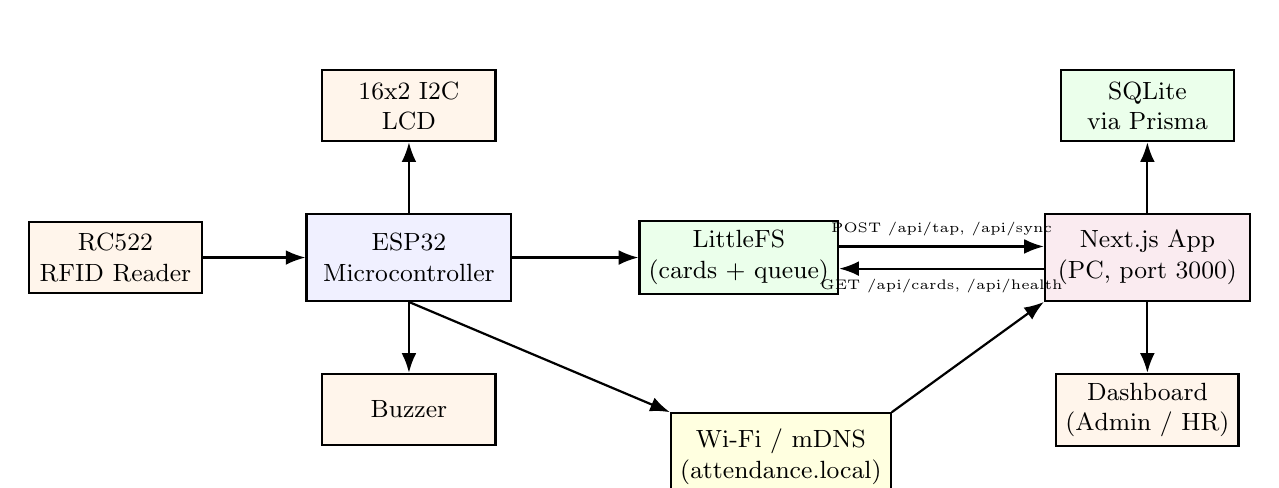
\begin{tikzpicture}[
        block/.style={rectangle, draw=black, thick, minimum width=2.6cm, minimum height=1.1cm, align=center, fill=blue!6, font=\small},
        io/.style={rectangle, draw=black, thick, minimum width=2.2cm, minimum height=0.9cm, align=center, fill=orange!8, font=\small},
        store/.style={rectangle, draw=black, thick, minimum width=2.2cm, minimum height=0.9cm, align=center, fill=green!8, font=\small},
        arrow/.style={-{Latex[length=2.5mm]}, thick},
        node distance=0.9cm and 1.3cm
    ]
        % ESP32 side
        \node[io] (rfid) {RC522\\RFID Reader};
        \node[block, right=of rfid] (esp32) {ESP32\\Microcontroller};
        \node[io, above=of esp32] (lcd) {16x2 I2C\\LCD};
        \node[io, below=of esp32] (buzzer) {Buzzer};
        \node[store, right=1.6cm of esp32] (flash) {LittleFS\\(cards + queue)};

        % Network
        \node[block, below right=1.4cm and 2.0cm of esp32, fill=yellow!12] (wifi) {Wi-Fi / mDNS\\(attendance.local)};

        % Server side
        \node[block, right=2.6cm of flash, fill=purple!8] (nextjs) {Next.js App\\(PC, port 3000)};
        \node[store, above=of nextjs] (sqlite) {SQLite\\via Prisma};
        \node[io, below=of nextjs] (dashboard) {Dashboard\\(Admin / HR)};

        \draw[arrow] (rfid) -- (esp32);
        \draw[arrow] (esp32) -- (lcd);
        \draw[arrow] (esp32) -- (buzzer);
        \draw[arrow] (esp32) -- (flash);
        \draw[arrow] (esp32.south) -- (wifi.north west);
        \draw[arrow] (wifi.north east) -- (nextjs.south west);
        \draw[arrow] (nextjs) -- (sqlite);
        \draw[arrow] (nextjs) -- (dashboard);

        \draw[arrow] ([yshift=4pt]flash.east) -- node[above, font=\tiny] {POST /api/tap, /api/sync} ([yshift=4pt]nextjs.west);
        \draw[arrow] ([yshift=-4pt]nextjs.west) -- node[below, font=\tiny] {GET /api/cards, /api/health} ([yshift=-4pt]flash.east);
    \end{tikzpicture}
    \caption{High-level system architecture: the ESP32 reader station always initiates contact with the PC application, never the other way around.}
    \label{fig:block-diagram}
\end{figure}

Two design choices in this diagram are worth calling out explicitly, because they are the parts of the architecture that differ from a typical class-project implementation:

\begin{itemize}
    \item \textbf{The ESP32 always initiates.} The PC application never opens a connection to the device. This keeps the device side simple, since it needs no server of its own, and means the PC can sit behind a firewall or NAT without any port-forwarding.
    \item \textbf{LittleFS sits between the reader and the network.} Every tap is written to flash before the device even attempts to send it. If that send fails, the tap is already safe and simply waits in a queue.
\end{itemize}

\section{Requirements Analysis}

\subsection{Functional Requirements}
\begin{itemize}
    \item Read a unique identifier from an RFID card presented to the reader.
    \item Distinguish a known card from an unknown one, using a locally cached list that works even without a network connection.
    \item Record the first tap of the day for a known card as an arrival, and the second as a departure, for whichever event is currently active.
    \item Give immediate audible and visual feedback at the reader for every tap, including the specific case of an unknown card.
    \item Allow an administrator to create students, create and end attendance events, and register a card from an unknown-tap alert.
    \item Display live Present / Left / Absent status for every student against the active event.
\end{itemize}

\subsection{Non-Functional Requirements}
\begin{itemize}
    \item \textbf{Availability:} the reader station must keep logging taps even if Wi-Fi or the PC application is unreachable.
    \item \textbf{Low latency:} a tap should be acknowledged at the reader (beep, LCD message) in well under a second.
    \item \textbf{Low cost:} the hardware bill of materials should stay well below the cost of a commercial RFID attendance terminal.
    \item \textbf{Maintainability:} the PC application must be installable and runnable by someone without a database administration background, given SQLite requires no separate server process.
    \item \textbf{Security:} unknown cards must never be auto-registered, to prevent an unauthorised card from silently gaining access to the attendance record.
\end{itemize}

\section{Hardware Design}
\label{sec:hardware-design}

\subsection{Component Selection}

Table~\ref{tab:component-summary} summarises the core components used in the reader station, and the subsections that follow explain the reasoning behind each choice in more detail.

\begin{table}[H]
    \centering
    \caption{Core hardware components}
    \label{tab:component-summary}
    \begin{tabular}{@{}p{3.2cm}p{9.5cm}@{}}
        \toprule
        \textbf{Component} & \textbf{Role in the system} \\
        \midrule
        ESP32-WROOM-32 DevKit & Main microcontroller: runs the firmware, drives every other component \\
        MFRC522 RFID reader & Reads the 13.56\,MHz UID from each employee's card \\
        16x2 I2C LCD & Gives on-the-spot feedback (name, "welcome", "unknown card", status) \\
        Active buzzer & Audible confirmation, distinct beep patterns per outcome \\
        Status LEDs (x2) & Wi-Fi connected / App reachable indicators \\
        Push button & Non-destructive local reset (clears sync queue, re-pulls card cache) \\
        LM2596 buck converter & Steps the 12\,V supply down to the voltages the reader circuit needs \\
        12\,V/2\,A power adapter & Mains power source for the enclosure \\
        Custom PCB & Carries all of the above cleanly instead of loose breadboard wiring \\
        \bottomrule
    \end{tabular}
\end{table}

\subsubsection{ESP32-WROOM-32 Development Board}

\begin{figure}[H]
    \centering
    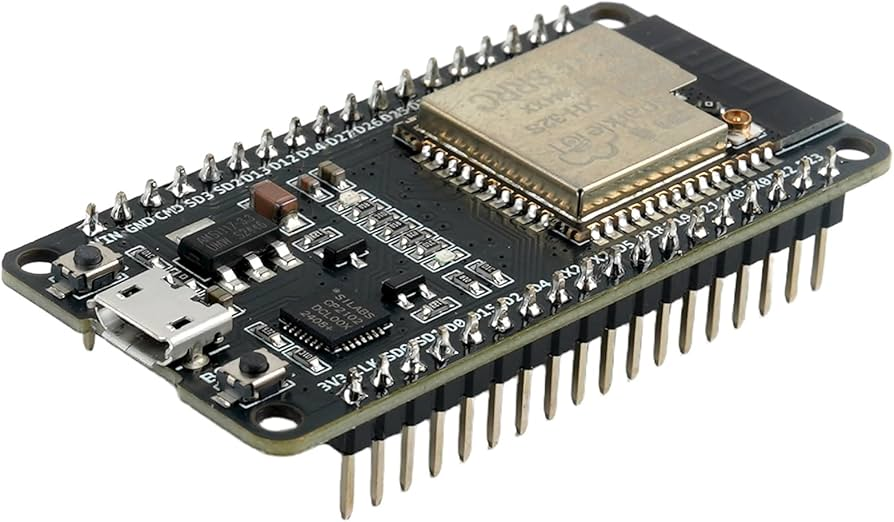
\includegraphics[width=0.55\textwidth]{esp32.jpg}
    \caption{ESP32-WROOM-32 development board used as the reader station's microcontroller}
    \label{fig:esp32}
\end{figure}

The ESP32 was chosen over a plain Arduino because it has built-in Wi-Fi, which the whole architecture in Section~\ref{sec:hardware-design} depends on — an Arduino Uno would have needed a separate Wi-Fi shield and more wiring for no real benefit. It also has enough GPIO pins to drive the RFID reader over SPI, the LCD over I2C, two LEDs, a buzzer, and a reset button at the same time without needing an I/O expander, and it is inexpensive enough that the whole reader station stays well within a modest project budget \parencite{espressif2023esp32}.

\subsubsection{MFRC522 RFID Reader Module}

\begin{figure}[H]
    \centering
    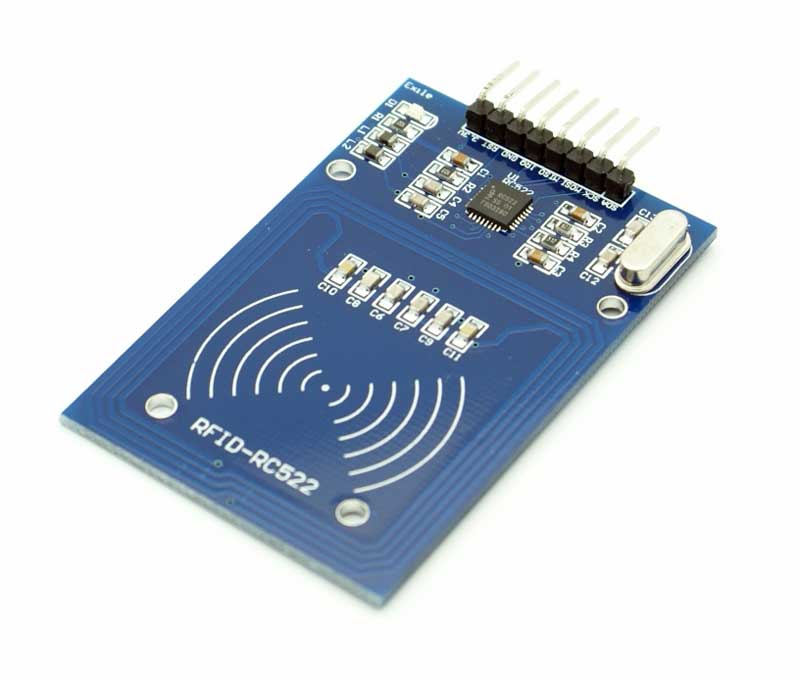
\includegraphics[width=0.5\textwidth]{rc522.jpg}
    \caption{MFRC522 RFID reader module}
    \label{fig:rc522}
\end{figure}

The MFRC522 is one of the most widely documented RFID front-end chips available to hobbyist and student projects, with a mature Arduino/ESP32 library and a well-specified datasheet \parencite{nxp2016mfrc522}. It communicates over SPI, reads 13.56\,MHz MIFARE-family cards at a range of a few centimetres, and — importantly for this project's budget — costs only a few dollars per unit. Its main limitation is that it must be powered from 3.3\,V rather than 5\,V, a detail that shaped the power-supply design discussed in Section~\ref{sec:power-design}.

\subsubsection{16x2 I2C LCD Display}

\begin{figure}[H]
    \centering
    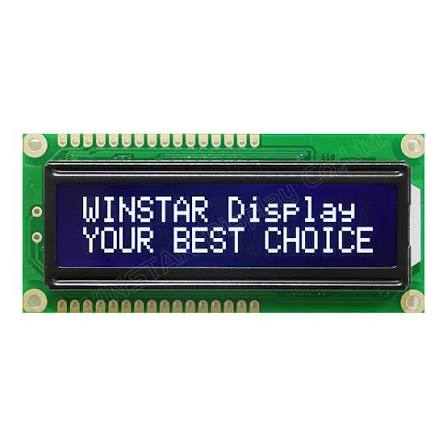
\includegraphics[width=0.45\textwidth]{lcd.jpg}
    \caption{16x2 character LCD with I2C (PCF8574) backpack}
    \label{fig:lcd}
\end{figure}

An LCD was chosen over relying on LEDs alone because a name or a short message ("Welcome, Dennis", "Unknown card, see front desk") is far more useful at the point of tap than a blinking light. The I2C backpack version was selected specifically because it reduces the wiring from the roughly ten pins a raw HD44780 panel needs down to just two data lines (SDA/SCL) plus power and ground, which mattered once the layout moved onto a compact custom PCB.

\subsubsection{Active Buzzer}

\begin{figure}[H]
    \centering
    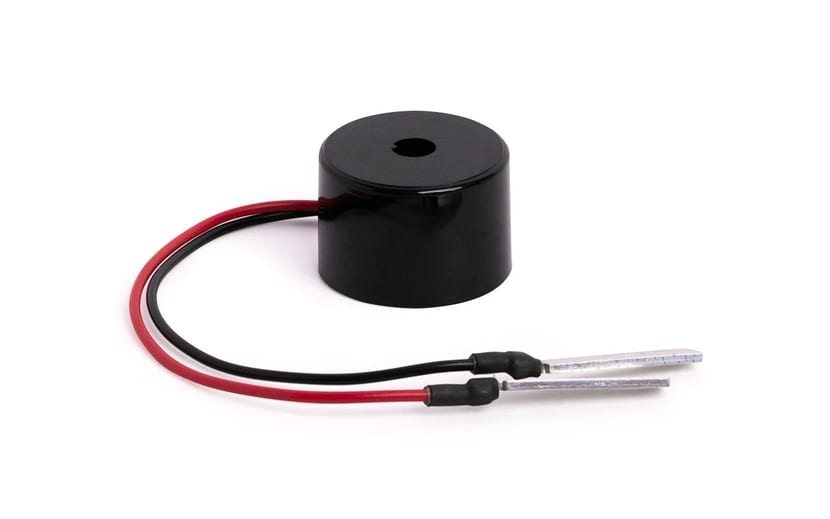
\includegraphics[width=0.4\textwidth]{buzzer.jpg}
    \caption{Active buzzer used for audible tap feedback}
    \label{fig:buzzer}
\end{figure}

The buzzer gives staff a way to confirm a tap succeeded without needing to look at the LCD every time. An \textit{active} buzzer was chosen over a passive one because it only needs a digital HIGH/LOW signal to produce a tone, rather than a driven PWM waveform — this keeps the firmware's \texttt{beep()} routine (Appendix~\ref{app:firmware}) a simple digitalWrite loop, and it is what allows different tap outcomes to be distinguished by beep count and timing alone: two short beeps for a normal tap, three for an already-recorded duplicate, and one long beep for an unknown card or a missing active event.

\subsubsection{Status LEDs}

\begin{figure}[H]
    \centering
    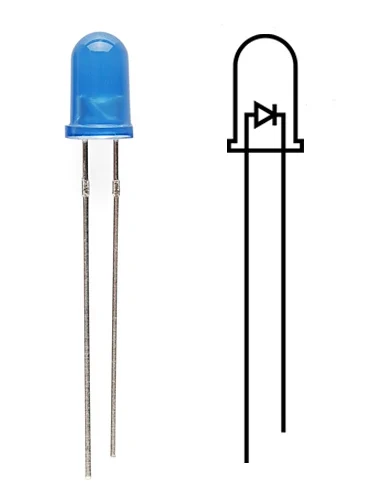
\includegraphics[width=0.28\textwidth]{LED.png}
    \caption{5\,mm LED, used for the Wi-Fi and App status indicators}
    \label{fig:led}
\end{figure}

Two identical 5\,mm LEDs were used, wired to separate GPIO pins so their meaning could be kept semantically distinct: one shows whether the device has joined the Wi-Fi network, the other shows whether the PC application actually responded to the last health check. This distinction was made deliberately, because "no Wi-Fi" and "Wi-Fi is fine but the server is unreachable" require different fixes, and a single combined status LED cannot tell front-desk staff which one they are dealing with.

\subsubsection{Power Supply: 12\,V Adapter and LM2596 Buck Converter}
\label{sec:power-design}

\begin{figure}[H]
    \centering
    \begin{subfigure}[b]{0.47\textwidth}
        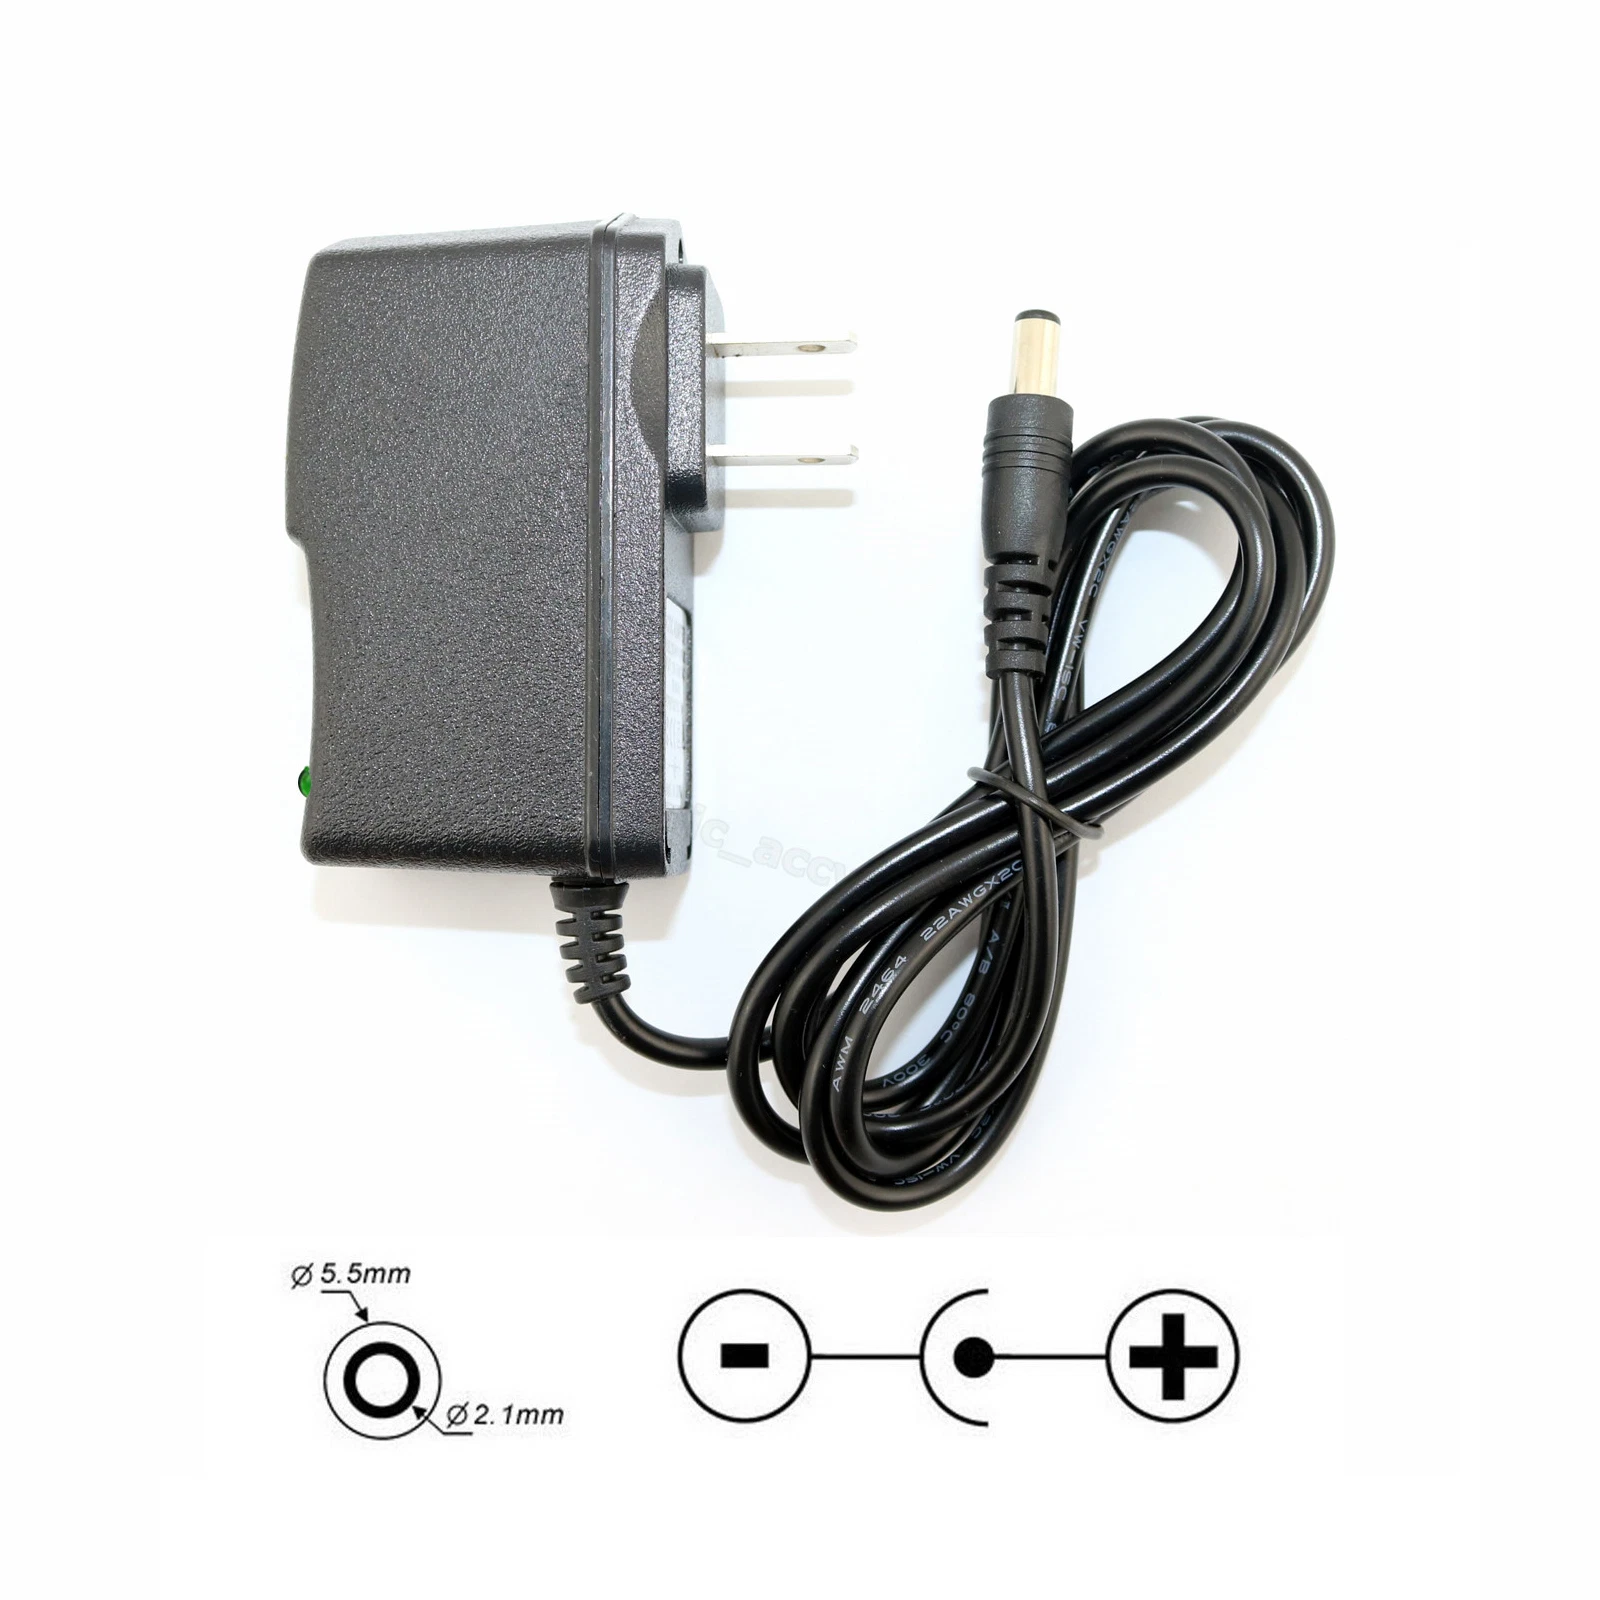
\includegraphics[width=\textwidth]{power_supply.png}
        \caption{12\,V/2\,A mains adapter}
    \end{subfigure}
    \hfill
    \begin{subfigure}[b]{0.47\textwidth}
        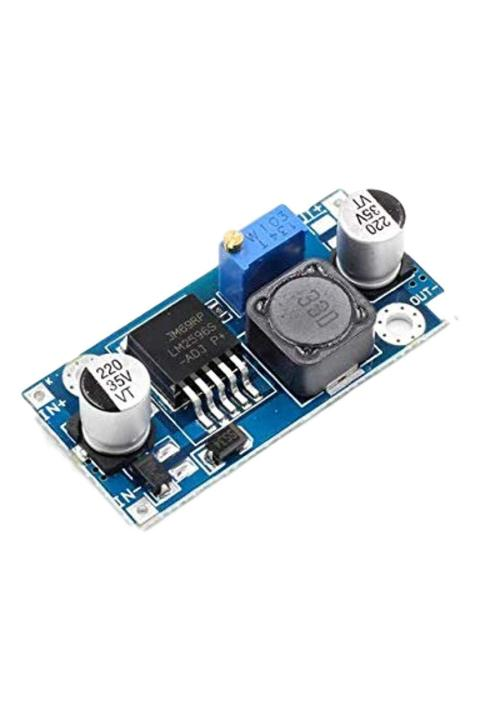
\includegraphics[width=\textwidth]{buck_coverter.jpg}
        \caption{LM2596 adjustable buck converter}
    \end{subfigure}
    \caption{Power supply components: a mains adapter feeding an adjustable buck converter}
    \label{fig:power-supply}
\end{figure}

A standard 12\,V/2\,A wall adapter supplies the enclosure, chosen because it is a common, inexpensive, and easily replaceable part rather than a custom power brick. Since neither the ESP32 board (5\,V in) nor its 3.3\,V logic rail can be fed 12\,V directly, an LM2596-based buck converter steps that down to a safe, regulated 5\,V before it reaches the ESP32's own onboard regulator. This two-stage approach — mains adapter to 5\,V, then the ESP32's own regulator to 3.3\,V for the logic rail — follows the voltage budget worked out during design: the RC522 must only ever see 3.3\,V, never 5\,V, since running it at 5\,V risks damaging the chip, while the LCD panel and its backlight are happy at 5\,V. The full voltage and current budget for every component is documented alongside the pinout table in Appendix~\ref{app:pinout}.

\subsection{Circuit Design}

The schematic in Figure~\ref{fig:schematic} was drawn in Proteus Design Suite before any PCB layout work began, so that every connection could be checked on paper first. It groups the RC522 reader, the LCD, the status LEDs and buzzer, and the ESP32 itself into clearly labelled blocks, with decoupling capacitors placed close to the power pins of the RC522 and the LCD to keep their supply rails stable during a card read.

\begin{figure}[H]
    \centering
    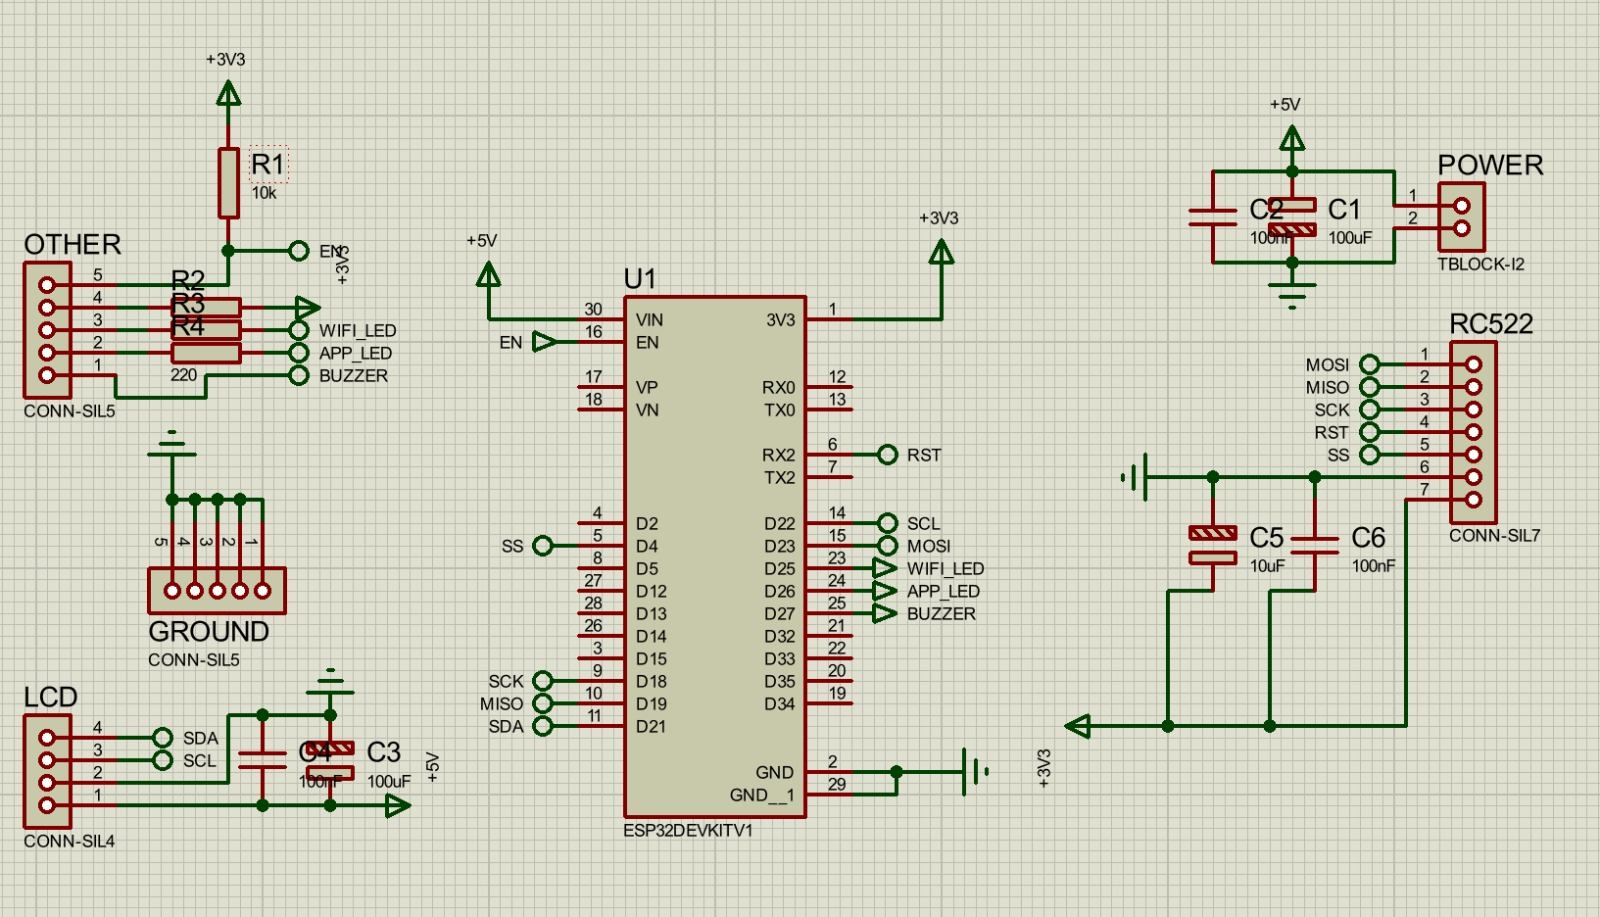
\includegraphics[width=\textwidth]{proteus_schematic_view.jpeg}
    \caption{Circuit schematic for the reader station, drawn in Proteus Design Suite}
    \label{fig:schematic}
\end{figure}

\subsection{PCB Design}

Once the schematic was verified, it was translated into a custom two-layer PCB layout (Figure~\ref{fig:pcb-layout}), rather than leaving the final build on a breadboard or stripboard. A custom board was worth the extra design time for three reasons: it removes the risk of a loose jumper wire causing an intermittent fault after the enclosure is closed up and installed at the entrance, it gives clearly labelled header positions for the RC522, LCD, and status components so the unit could be reassembled or repaired without re-deriving the wiring from scratch, and it fits inside a much smaller enclosure than an equivalent breadboard build. Figure~\ref{fig:pcb-3d} shows the resulting layout rendered in 3D, with the ESP32 DevKit mounted directly onto the board via pin headers.

\begin{figure}[H]
    \centering
    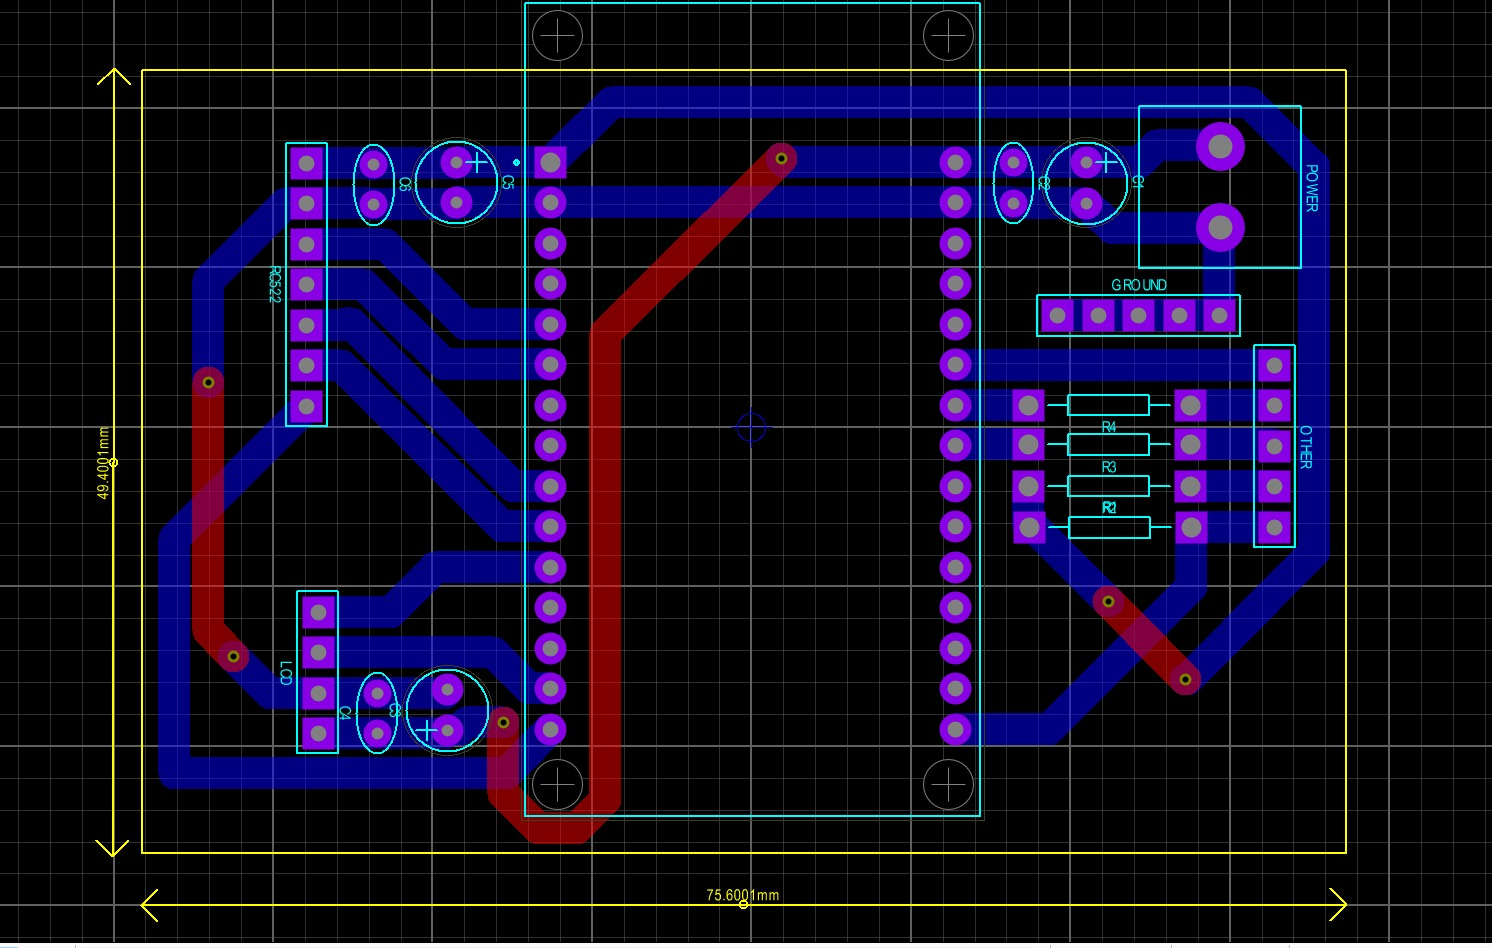
\includegraphics[width=0.85\textwidth]{proteus_pcb_view.jpeg}
    \caption{PCB layout (top copper in blue, bottom copper in purple) for the reader station}
    \label{fig:pcb-layout}
\end{figure}

\begin{figure}[H]
    \centering
    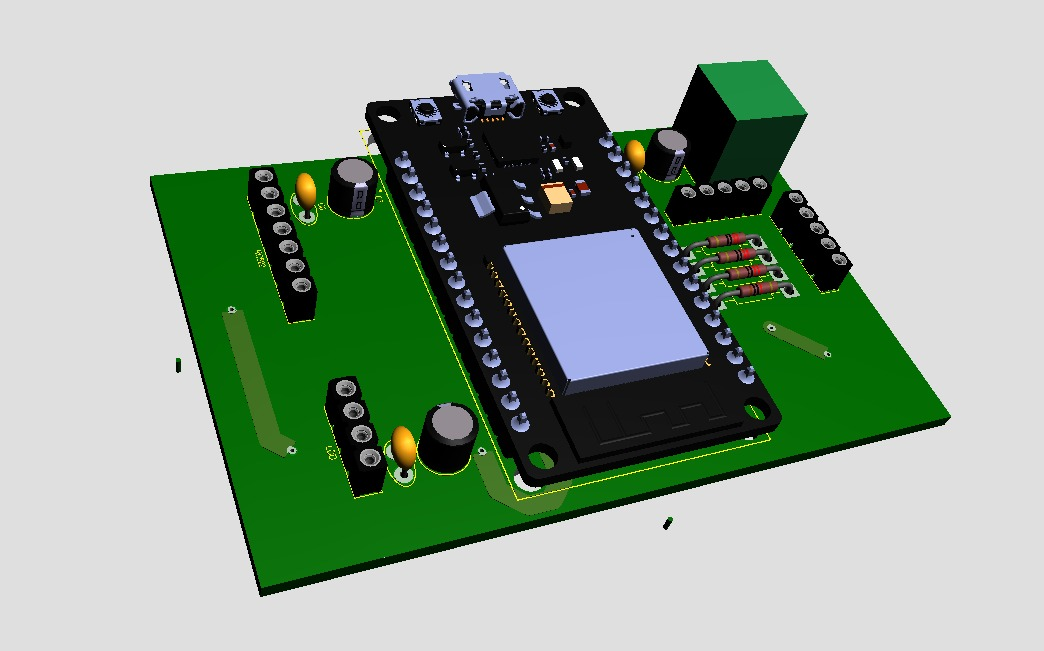
\includegraphics[width=0.7\textwidth]{proteus_pcb_3d.jpeg}
    \caption{3D render of the assembled reader station PCB}
    \label{fig:pcb-3d}
\end{figure}

\section{Firmware Design}

The ESP32 firmware (the full source is reproduced in Appendix~\ref{app:firmware}) is built around a single non-blocking \texttt{loop()} that checks the reset button, maintains the Wi-Fi and server connection, polls the RFID reader, drains the offline queue when possible, and refreshes the idle LCD screen — all on every pass, none of them waiting on the others. The logic that matters most for the objectives in Chapter 1 is what happens the instant a card is tapped, shown in Figure~\ref{fig:tap-flowchart}.

\begin{figure}[H]
    \centering
    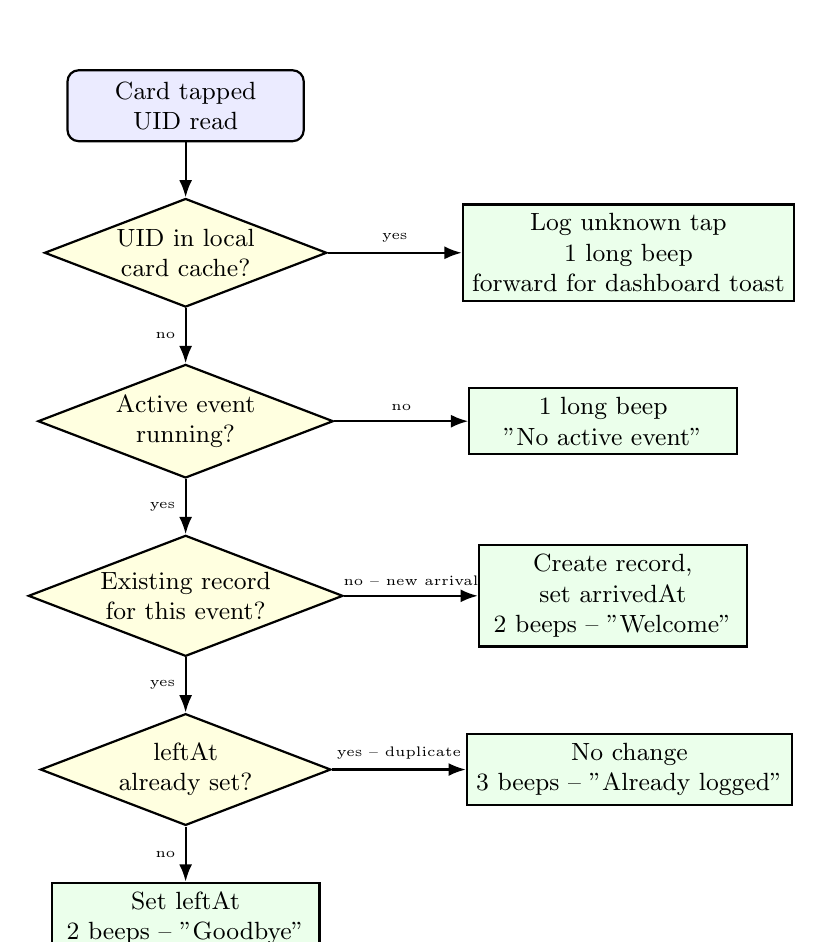
\begin{tikzpicture}[
        node distance=0.7cm and 1.7cm,
        startstop/.style={rectangle, rounded corners, draw=black, thick, fill=blue!8, minimum width=3.0cm, minimum height=0.9cm, align=center, font=\small},
        decision/.style={diamond, draw=black, thick, fill=yellow!12, aspect=2.6, inner sep=1pt, align=center, font=\small},
        process/.style={rectangle, draw=black, thick, fill=green!8, minimum width=3.4cm, minimum height=0.8cm, align=center, font=\small},
        arrow/.style={-{Latex[length=2.2mm]}, thick}
    ]
        \node[startstop] (start) {Card tapped\\UID read};
        \node[decision, below=of start] (known) {UID in local\\card cache?};
        \node[decision, below=of known] (activeevt) {Active event\\running?};
        \node[decision, below=of activeevt] (hasrecord) {Existing record\\for this event?};
        \node[decision, below=of hasrecord] (hasleft) {leftAt\\already set?};
        \node[process, below=of hasleft] (depart) {Set leftAt\\2 beeps -- "Goodbye"};

        \node[process, right=of known] (unknown) {Log unknown tap\\1 long beep\\forward for dashboard toast};
        \node[process, right=of activeevt] (noevt) {1 long beep\\"No active event"};
        \node[process, right=of hasrecord] (arrive) {Create record,\\set arrivedAt\\2 beeps -- "Welcome"};
        \node[process, right=of hasleft] (dup) {No change\\3 beeps -- "Already logged"};

        \draw[arrow] (start) -- (known);
        \draw[arrow] (known) -- node[left, font=\tiny]{no} (activeevt);
        \draw[arrow] (known) -- node[above, font=\tiny]{yes} (unknown);
        \draw[arrow] (activeevt) -- node[left, font=\tiny]{yes} (hasrecord);
        \draw[arrow] (activeevt) -- node[above, font=\tiny]{no} (noevt);
        \draw[arrow] (hasrecord) -- node[left, font=\tiny]{yes} (hasleft);
        \draw[arrow] (hasrecord) -- node[above, font=\tiny]{no -- new arrival} (arrive);
        \draw[arrow] (hasleft) -- node[left, font=\tiny]{no} (depart);
        \draw[arrow] (hasleft) -- node[above, font=\tiny]{yes -- duplicate} (dup);
    \end{tikzpicture}
    \caption{Tap-handling logic, shared identically between the live \texttt{/api/tap} path and the offline queue replayed through \texttt{/api/sync}. The main decision spine runs top to bottom; each outcome branches right to the resulting beep/LCD feedback and database action.}
    \label{fig:tap-flowchart}
\end{figure}

Note that the decision "UID in local card cache?" is answered entirely from the copy of the card list stored on the ESP32's own flash — the device never needs to ask the server whether a card is known before giving feedback. That cache is refreshed periodically from \texttt{GET /api/cards} whenever the app is reachable, which is what allows a newly registered student to start tapping in successfully within about a minute of being added on the dashboard, even if the reader briefly loses connectivity right after.

\section{Software Architecture}

The PC application is built with Next.js, using its API routes to expose the endpoints in Table~\ref{tab:api-endpoints} to the ESP32, and its page routes for the dashboard, students, and events screens used by staff. Every tap — whether delivered live or replayed from the device's offline queue — is processed through one shared function, so the arrival/departure/duplicate rules in Figure~\ref{fig:tap-flowchart} cannot drift out of sync between the two code paths.

\begin{table}[H]
    \centering
    \caption{API endpoints exposed by the PC application}
    \label{tab:api-endpoints}
    \begin{tabular}{@{}p{2.6cm}p{3.6cm}p{6.5cm}@{}}
        \toprule
        \textbf{Method} & \textbf{Endpoint} & \textbf{Purpose} \\
        \midrule
        GET & /api/health & Liveness check used to drive the App-reachable LED \\
        POST & /api/tap & Submit a single live tap (UID, timestamp) \\
        POST & /api/sync & Submit a batch of queued taps after reconnecting \\
        GET & /api/cards & Return all known card UIDs, for the device's local cache \\
        \bottomrule
    \end{tabular}
\end{table}

A full list of the application's routes, including the student- and event-management endpoints used only by the dashboard itself, is given in Appendix~\ref{app:api}.

\section{Database Design}

Attendance status is deliberately \textit{not} stored as a field anywhere in the database. Instead, it is computed on every request from two nullable timestamps, as shown in the entity-relationship diagram in Figure~\ref{fig:erd}. A student with no attendance record at all for the active event is \textit{Absent}; a record with \texttt{arrivedAt} set but \texttt{leftAt} still null is \textit{Present}; a record with both set is \textit{Left}. This avoids the class of bug where a stored status field quietly falls out of sync with the timestamps it was supposed to summarise.

\begin{figure}[H]
    \centering
    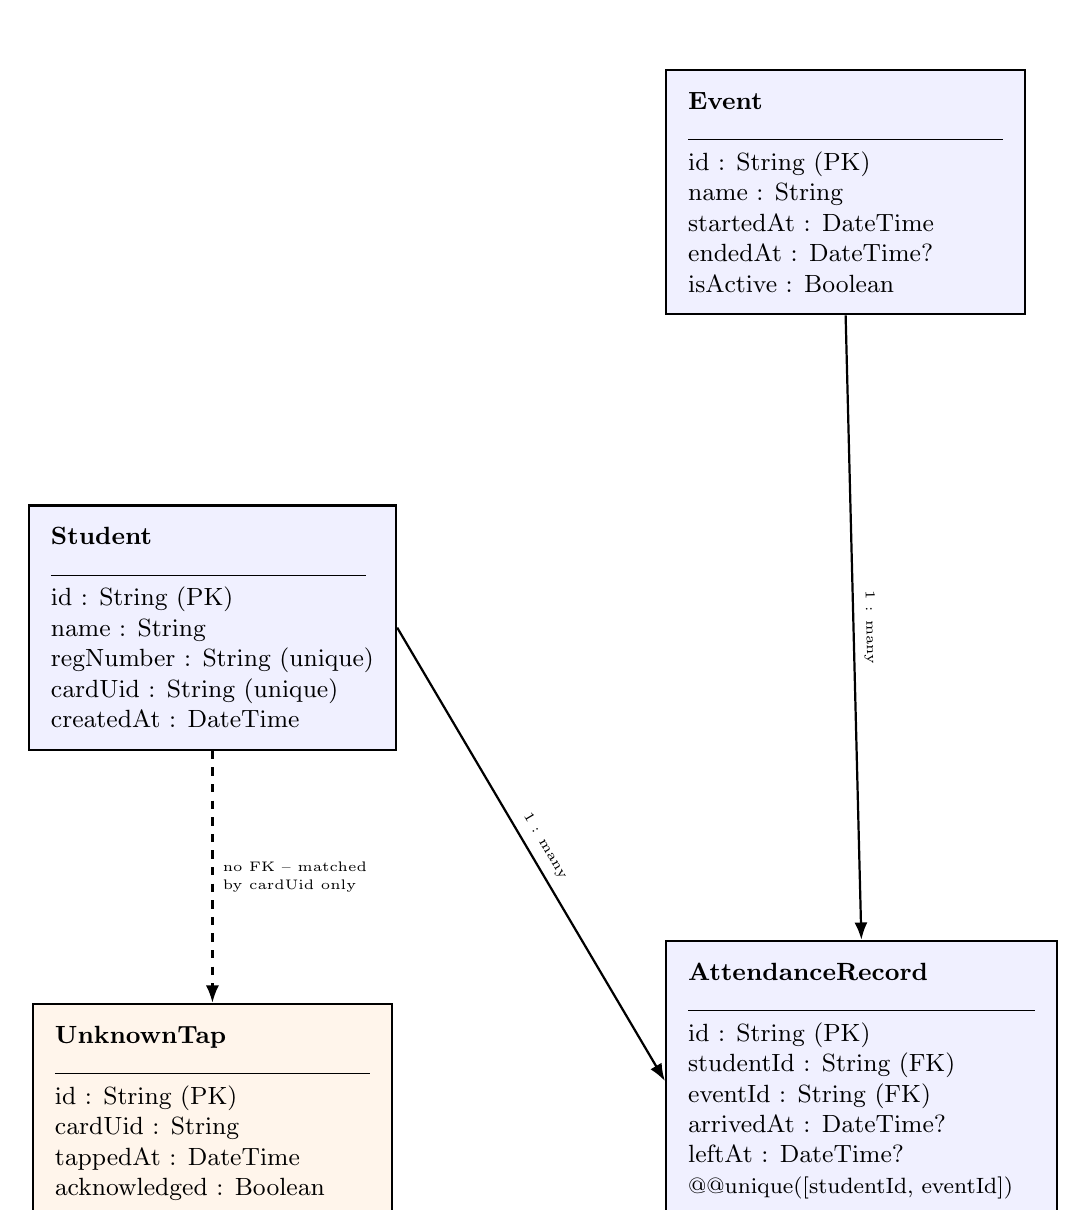
\begin{tikzpicture}[
        entity/.style={rectangle, draw=black, thick, fill=blue!6, minimum width=4.4cm, align=left, font=\small, inner sep=8pt},
        rel/.style={-{Latex[length=2.2mm]}, thick}
    ]
        \node[entity] (student) {
            \textbf{Student}\\
            \rule{4cm}{0.3pt}\\
            id : String (PK)\\
            name : String\\
            regNumber : String (unique)\\
            cardUid : String (unique)\\
            createdAt : DateTime
        };

        \node[entity, below right=2.4cm and 3.4cm of student] (record) {
            \textbf{AttendanceRecord}\\
            \rule{4.4cm}{0.3pt}\\
            id : String (PK)\\
            studentId : String (FK)\\
            eventId : String (FK)\\
            arrivedAt : DateTime?\\
            leftAt : DateTime?\\
            \footnotesize @@unique([studentId, eventId])
        };

        \node[entity, above right=2.4cm and 3.4cm of student] (event) {
            \textbf{Event}\\
            \rule{4cm}{0.3pt}\\
            id : String (PK)\\
            name : String\\
            startedAt : DateTime\\
            endedAt : DateTime?\\
            isActive : Boolean
        };

        \node[entity, below=3.2cm of student, fill=orange!8] (unknown) {
            \textbf{UnknownTap}\\
            \rule{4cm}{0.3pt}\\
            id : String (PK)\\
            cardUid : String\\
            tappedAt : DateTime\\
            acknowledged : Boolean
        };

        \draw[rel] (student.east) -- node[above, sloped, font=\tiny]{1 : many} (record.west);
        \draw[rel] (event.south) -- node[above, sloped, font=\tiny]{1 : many} (record.north);
        \draw[rel, dashed] (student.south) -- node[right, font=\tiny]{\shortstack[l]{no FK -- matched\\by cardUid only}} (unknown.north);
    \end{tikzpicture}
    \caption{Entity-relationship diagram of the Prisma/SQLite data model. UnknownTap has no foreign key to Student because, by definition, no matching student exists yet.}
    \label{fig:erd}
\end{figure}

\section{Bill of Quantities}

Table~\ref{tab:boq} lists the components purchased for a single reader station, with approximate unit prices in United States Dollars based on prevailing local electronics-supplier prices at the time of purchase. Prices are indicative and will vary by supplier and by the quantity ordered.

\begin{table}[H]
    \centering
    \caption{Bill of Quantities for one reader station}
    \label{tab:boq}
    \begin{tabular}{@{}p{5.2cm}ccrr@{}}
        \toprule
        \textbf{Item} & \textbf{Unit} & \textbf{Qty} & \textbf{Unit Price (USD)} & \textbf{Total (USD)} \\
        \midrule
        ESP32-WROOM-32 DevKit & pc & 1 & 6.00 & 6.00 \\
        MFRC522 RFID reader module & pc & 1 & 2.50 & 2.50 \\
        13.56\,MHz Mifare RFID cards & pc & 10 & 0.50 & 5.00 \\
        16x2 I2C LCD display & pc & 1 & 3.50 & 3.50 \\
        Active buzzer module & pc & 1 & 0.80 & 0.80 \\
        5\,mm LEDs (status indicators) & pc & 2 & 0.10 & 0.20 \\
        220\,$\Omega$ resistors & pc & 4 & 0.05 & 0.20 \\
        Momentary push button & pc & 1 & 0.30 & 0.30 \\
        LM2596 buck converter module & pc & 1 & 1.50 & 1.50 \\
        12\,V / 2\,A mains power adapter & pc & 1 & 4.00 & 4.00 \\
        Custom 2-layer PCB (fabrication, qty 3) & lot & 1 & 15.00 & 15.00 \\
        Weatherproof enclosure box & pc & 1 & 5.00 & 5.00 \\
        Header pins, wiring, solder, misc. & lot & 1 & 3.00 & 3.00 \\
        \midrule
        \multicolumn{4}{r}{\textbf{Total}} & \textbf{47.00} \\
        \bottomrule
    \end{tabular}
\end{table}

No cost is attributed to the PC running the Next.js application, since Infor Relay Systems (Pvt) Ltd already had a suitable front-desk computer available; the software itself uses only free and open-source tools.

\section{Testing Approach}

Testing followed the same incremental order the system was built in. The RC522 was first tested in isolation with a simple UID-dump sketch to confirm reliable reads before any other component was wired in. The buzzer and LED patterns were then verified against the beep table in Figure~\ref{fig:tap-flowchart} using test button presses, without any network code running. The LittleFS card cache and offline queue were tested by physically disconnecting the reader station's Wi-Fi mid-session and confirming that taps were still saved and later drained once connectivity returned. Finally, the complete system was tested end-to-end during a live orientation-day event at Infor Relay Systems (Pvt) Ltd, tapping in and out with several registered cards and one deliberately unregistered card to confirm the unknown-card alert and registration flow. The results of that testing are presented in Chapter 4.

\chapter{Results}
\label{ch:results}

\section{Introduction}

This chapter presents the finished system as it was tested and demonstrated at Infor Relay Systems (Pvt) Ltd, and then evaluates it directly against the three objectives set out in Chapter 1. Screenshots throughout this chapter were captured during a live test event, run on-site to confirm the whole pipeline — card tap, reader feedback, network delivery, and dashboard update — worked together outside of the lab setting it was developed in.

\section{The Finished Hardware}

Figure~\ref{fig:finished-hardware} shows the assembled reader station in its enclosure, built on the custom PCB described in Chapter 3. The LCD sits at the top for at-a-glance feedback, with the two status LEDs mounted directly beneath it and the RFID reader positioned behind the front face of the enclosure, immediately below the printed tap icon, so a card only needs to be held against that marked area to register a read.

\begin{figure}[H]
    \centering
    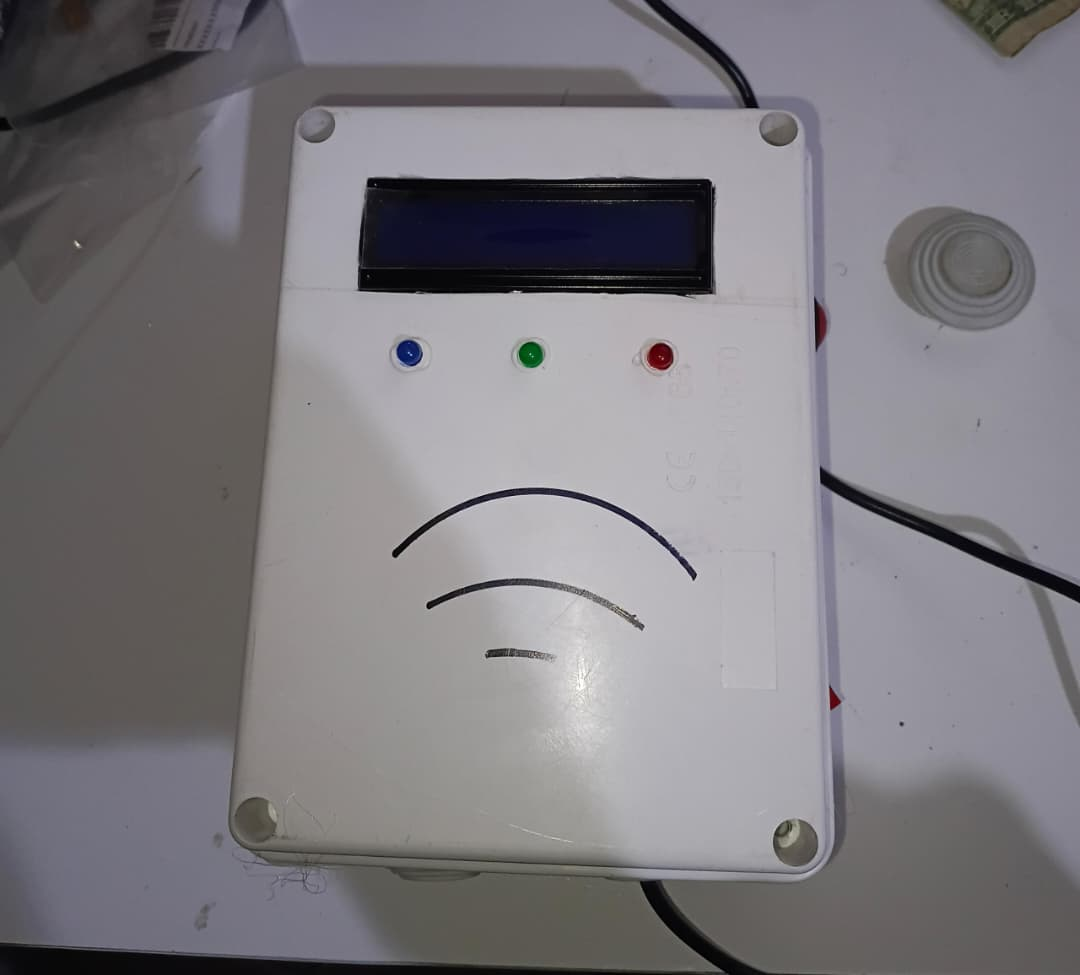
\includegraphics[width=0.5\textwidth]{finished_hardware.jpeg}
    \caption{The completed reader station, enclosed and ready for deployment at the entrance}
    \label{fig:finished-hardware}
\end{figure}

\section{The Dashboard Application}

\subsection{Events}

Figure~\ref{fig:events-screenshot} shows the Events screen used to start and end an attendance period. For the on-site test, an event named "Orientation day" was started at 07:41:30 on 14 August 2026; every tap recorded afterwards was automatically attributed to this event until it was explicitly ended, matching the event-lifecycle behaviour described in Chapter 3.

\begin{figure}[H]
    \centering
    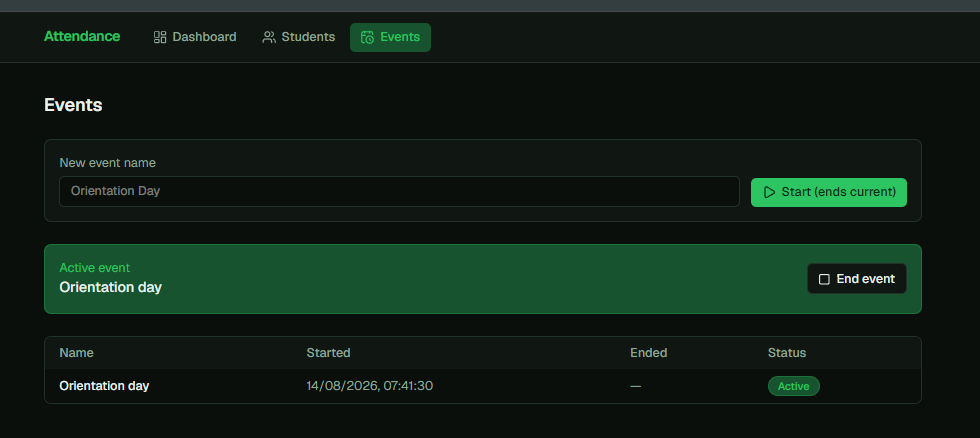
\includegraphics[width=0.85\textwidth]{events.png}
    \caption{Events screen: creating and monitoring the active attendance event}
    \label{fig:events-screenshot}
\end{figure}

\subsection{Student Registration}

Figure~\ref{fig:students-screenshot} shows the Students screen, where each employee is registered with a name, a registration number, and the UID of the card issued to them. Three students were registered for the test: Dennis (card UID \texttt{AAC06606}), Hwinza (\texttt{53EAB814}), and Job (\texttt{539CF8F4}). This is also the screen an administrator is taken to when they act on an unknown-card alert from the dashboard, with the scanned UID pre-filled so it does not need to be typed in by hand.

\begin{figure}[H]
    \centering
    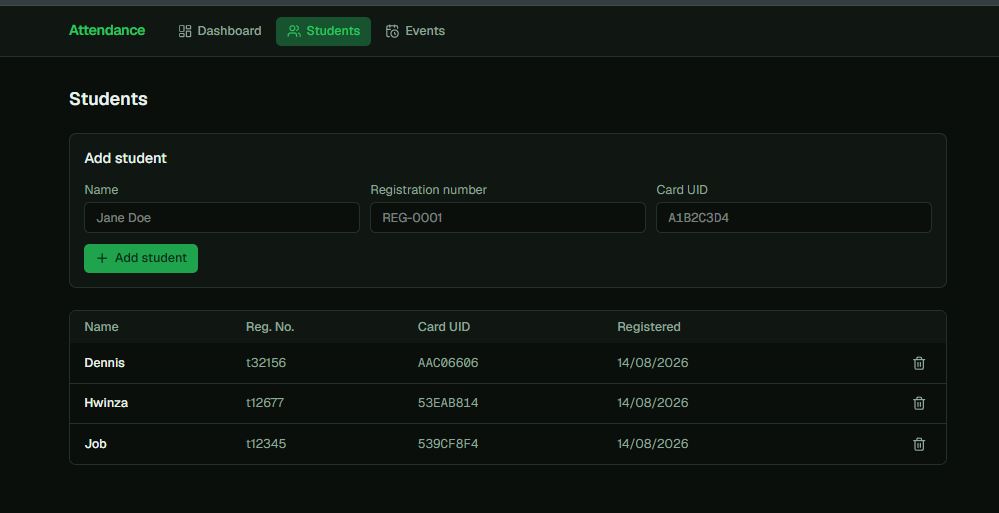
\includegraphics[width=0.85\textwidth]{students.png}
    \caption{Students screen: registering a card UID against a name and registration number}
    \label{fig:students-screenshot}
\end{figure}

\subsection{Live Attendance Dashboard}

Figure~\ref{fig:dashboard-screenshot} shows the dashboard partway through the test event. Dennis had tapped in at 07:41:47 and not yet tapped out, so he is shown as \textit{Present}. Hwinza and Job had each tapped in and then out again, so both are shown as \textit{Left}, with their exact arrival and departure times recorded to the second. No student shows as \textit{Absent} in this view because all three registered cards had been tapped at least once by the time the screenshot was taken.

\begin{figure}[H]
    \centering
    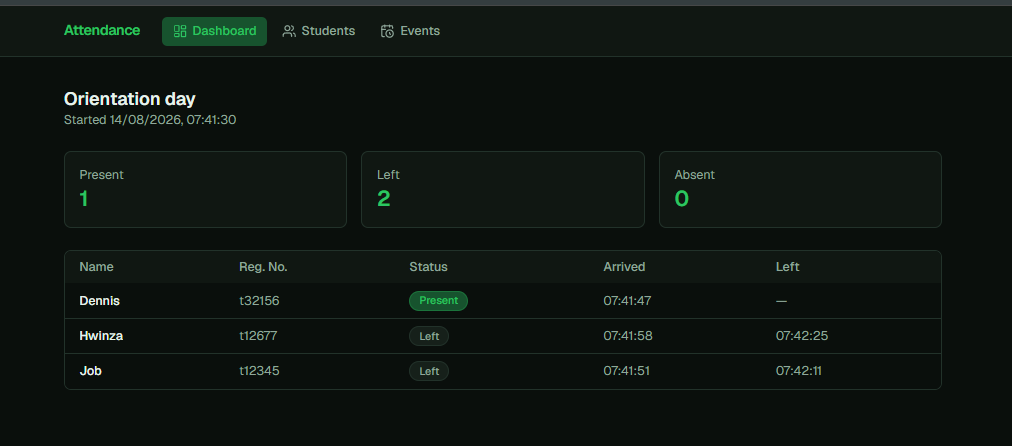
\includegraphics[width=0.85\textwidth]{dashboard.png}
    \caption{Live dashboard for the active event, showing computed Present / Left / Absent status per student}
    \label{fig:dashboard-screenshot}
\end{figure}

\section{Evaluation Against Objectives}

\subsection{Objective 1: Automating Attendance Tracking}

This objective was achieved. Figure~\ref{fig:dashboard-screenshot} demonstrates arrival and departure being captured automatically, to the second, with no manual data entry involved beyond the initial one-time registration of each card in Figure~\ref{fig:students-screenshot}. The tap-handling logic in Figure~\ref{fig:tap-flowchart} runs identically whether the reader is online or replaying a queued tap from its offline store, so the same automation holds even through a network interruption — the specific failure mode manual registers and always-online competitor systems alike do not handle gracefully, as discussed in Chapter 2.

\subsection{Objective 2: Ensuring Accurate Labour Costing}

This objective was substantially achieved. The \texttt{arrivedAt} and \texttt{leftAt} timestamps visible in Figure~\ref{fig:dashboard-screenshot} are precise to the second and are written the moment a tap is processed, not reconstructed later from memory or a supervisor's estimate — directly addressing the "incorrect attendance records" and payroll-reconciliation problem identified in the Chapter 1 problem statement. What was not built during this attachment is an automatic hours-worked or wage calculation on top of those timestamps; the dashboard reports status and exact times, and a payroll clerk would still need to derive total hours from them, either manually or through a short script against the underlying data. That gap is carried forward as a recommendation in Chapter 5 rather than claimed as solved here.

\subsection{Objective 3: Integrating RFID Attendance with Existing Systems}

This objective was only partially achieved, and it is worth being direct about that rather than overstating the result. The system exposes its data through a documented set of API endpoints (Table~\ref{tab:api-endpoints}, Appendix~\ref{app:api}) and a SQLite database that any payroll or HR tool capable of making an HTTP request or reading a database file could, in principle, consume. However, no such integration with Infor Relay Systems (Pvt) Ltd's actual payroll process was implemented or tested within the scope of this attachment — the "existing systems" referred to in the original objective were not accessible for direct integration during the project timeline. What was achieved is a system that is architecturally ready for that integration, rather than one where the integration itself is complete. This distinction, and what a follow-up phase of integration work would involve, is discussed further in Chapter 5.

\section{Discussion}

Across the on-site test, the offline-first design held up as intended: taps made while the reader's App-reachable LED was off were confirmed, after the fact, to have been queued locally and delivered automatically once the PC application came back within reach, with no gap in the resulting attendance record. The two-LED status indicator also proved useful in practice during setup, immediately showing when the issue was a Wi-Fi credential problem rather than the Next.js application not yet being started on the PC — a distinction that would otherwise have taken longer to diagnose by trial and error.

Taken together, the results show a system that meets its core aim of automated, accurate, real-time attendance capture, with the labour-costing objective met at the data level and the systems-integration objective met at the architectural level but not yet in a live production integration. Both of the partially met objectives point directly to the recommendations set out in the next chapter.

\chapter{Conclusion and Recommendations}
\label{ch:conclusion}

\section{Conclusion}

This project set out to replace a paper attendance register at Infor Relay Systems (Pvt) Ltd with a system that captures arrival and departure automatically, accurately, and in a way that front-desk staff could trust even when the network was not cooperating. The Real-Time RFID Employee Attendance System built during this attachment does exactly that: an ESP32 reader station with an MFRC522 module captures each tap, stores it to local flash before attempting to forward it, and syncs automatically once connectivity returns; a Next.js application on a PC turns those taps into a live Present/Left/Absent dashboard backed by a small, well-structured SQLite database.

Chapter 4 showed that the first objective — automating attendance tracking — was fully achieved, and demonstrated with real taps during an on-site test event. The second objective, accurate labour costing, was substantially achieved: every timestamp needed to calculate hours worked is now captured automatically and precisely, even though the wage-calculation step itself was left for a payroll process outside this system. The third objective, integrating with existing systems, was met only at the architectural level — the API and database are ready to be consumed by a payroll or HR tool, but that integration was not built or tested during the attachment period. Reporting that honestly here, rather than overstating it, is intentional: it is exactly the kind of gap a reader of this report needs to know about before treating the system as production-complete.

More broadly, the project confirms what the literature in Chapter 2 suggested: RFID is a fast, inexpensive, and well-proven way to automate attendance capture, and the harder engineering problem is not reading the card, it is keeping the system trustworthy when the network cannot be relied on. Designing for that from the start — rather than adding it later — is the main technical contribution of this attachment project.

\section{Recommendations}

The following recommendations follow directly from the limitations identified in Chapters 1, 3, and 4, and from a number of design decisions that were deliberately left open during this attachment for a future iteration to settle:

\begin{enumerate}[label=\arabic*.]
    \item \textbf{Build the payroll/HR integration.} The API already exposes everything a payroll system would need; the next step is a direct feed — a scheduled export or a live API integration — into whichever payroll tool Infor Relay Systems (Pvt) Ltd uses, so Objective 3 moves from architecturally ready to fully delivered.
    \item \textbf{Add automatic hours-worked calculation.} A simple report that turns each student's \texttt{arrivedAt}/\texttt{leftAt} pair into total hours for a pay period would close the remaining gap in Objective 2 without requiring any change to the data already being captured.
    \item \textbf{Decide the duplicate-tap policy explicitly.} Currently, a third tap after both arrival and departure are recorded is acknowledged with a distinct beep but makes no change to the record. Whether a genuine re-entry (for example, leaving briefly and returning) should update the record is a policy decision for management, not a technical one, and should be settled before wider rollout.
    \item \textbf{Consider a second factor for higher-risk areas.} As discussed in Chapter 2, RFID alone cannot prevent a card being knowingly handed to a colleague. For entrances where that risk matters more, pairing the existing reader with a low-cost fingerprint module would close that gap without discarding the RFID infrastructure already built.
    \item \textbf{Scale to multiple entrances.} The architecture already supports this with no redesign — each additional reader station is simply another ESP32 talking to the same PC application — but it has not yet been tested with more than one station running concurrently.
    \item \textbf{Tune the card-cache and reset-button behaviour from real usage data.} The 60-second card-sync interval and the reset button's "clear queue and re-pull cards" behaviour were reasonable defaults chosen during development; both are worth revisiting once there is real deployment data on how often cards are registered and how often the reset button actually gets used.
\end{enumerate}

\section{Project Timeline}

Figure~\ref{fig:gantt} shows the schedule followed during the attachment, from initial problem analysis in early May through to final report writing in July. The literature review is shown running for the full duration of the project rather than as a single early task, since relevant sources — particularly around offline-first design patterns — continued to be consulted throughout implementation, not only at the planning stage.

\begin{figure}[H]
    \centering
    \begin{ganttchart}[
        hgrid,
        vgrid,
        x unit=0.62cm,
        y unit chart=0.7cm,
        bar/.append style={fill=blue!35},
        bar height=0.55,
        group/.append style={fill=orange!45},
        group height=0.55,
        title height=1,
        title label font=\scriptsize,
        bar label font=\scriptsize,
        group label font=\scriptsize\bfseries
    ]{1}{13}
        \gantttitle{May}{4}
        \gantttitle{June}{5}
        \gantttitle{July}{4} \\
        \gantttitlelist{1,...,13}{1} \\
        \ganttgroup{Literature Review}{1}{13} \\
        \ganttbar{Problem analysis \& requirements}{1}{2} \\
        \ganttbar{Component sourcing}{2}{3} \\
        \ganttbar{Circuit schematic (Proteus)}{3}{4} \\
        \ganttbar{PCB design \& fabrication}{4}{6} \\
        \ganttbar{Firmware: RFID, LCD, buzzer, LEDs}{5}{7} \\
        \ganttbar{Firmware: Wi-Fi, mDNS, offline queue}{7}{8} \\
        \ganttbar{Next.js API \& database}{6}{9} \\
        \ganttbar{Dashboard UI}{9}{10} \\
        \ganttbar{Hardware assembly \& enclosure}{8}{9} \\
        \ganttbar{Integration testing}{10}{11} \\
        \ganttbar{On-site deployment \& field testing}{11}{12} \\
        \ganttbar{Report writing}{11}{13}
    \end{ganttchart}
    \caption{Project Gantt chart, May to July, with the literature review spanning the full project duration}
    \label{fig:gantt}
\end{figure}


% =============================================================================
% BACK MATTER
% =============================================================================
\appendix
\chapter{ESP32 Firmware Source Code}
\label{app:firmware}

The complete Arduino sketch running on the reader station is reproduced below, exactly as flashed to the device. It implements the boot sequence, Wi-Fi and mDNS connection handling, RFID card reading, the offline tap queue on LittleFS, and the reset-button behaviour discussed in Chapter 3.

\lstinputlisting[
    language=C++,
    caption={\texttt{attendance-firmware.ino} -- full ESP32 reader station firmware},
    label={lst:firmware}
]{../attendance-firmware/attendance-firmware.ino}

\chapter{ESP32 Pinout and Power Budget}
\label{app:pinout}

\section*{Pinout Table}

Table~\ref{tab:pinout} lists every wired connection between the ESP32 and the rest of the reader station circuit. GPIO choices deliberately avoid the ESP32's input-only pins (34--39) and its boot-strapping pins (0, 2, 5, 12, 15), so nothing on this board can interfere with the module's boot sequence.

\begin{table}[H]
    \centering
    \caption{ESP32-WROOM-32 pin assignments}
    \label{tab:pinout}
    \begin{tabular}{@{}p{3.4cm}p{2.8cm}p{1.8cm}p{5.3cm}@{}}
        \toprule
        \textbf{Component} & \textbf{Pin on component} & \textbf{ESP32 GPIO} & \textbf{Notes} \\
        \midrule
        RC522 (RFID reader) & SDA (SS/CS) & GPIO 4 & Chip select, moved off GPIO 21 to free the I2C bus \\
        RC522 & SCK & GPIO 18 & VSPI clock (fixed) \\
        RC522 & MOSI & GPIO 23 & VSPI MOSI (fixed) \\
        RC522 & MISO & GPIO 19 & VSPI MISO (fixed) \\
        RC522 & IRQ & Not connected & Not used; polling mode \\
        RC522 & RST & GPIO 16 & Moved off GPIO 22 to free the I2C SCL \\
        RC522 & VCC & 3.3\,V & Must not be powered from 5\,V \\
        Wi-Fi status LED & Anode & GPIO 25 & Through current-limiting resistor \\
        App-reachable LED & Anode & GPIO 26 & Through current-limiting resistor \\
        Buzzer & Signal & GPIO 27 & Active buzzer, direct digital drive \\
        Reset button & One leg & GPIO 32 & \texttt{INPUT\_PULLUP}, active-low, other leg to GND \\
        LCD 16x2 I2C & SDA & GPIO 21 & I2C data line \\
        LCD 16x2 I2C & SCL & GPIO 22 & I2C clock line \\
        LCD 16x2 I2C & VCC & 5\,V & Powers panel and backlight \\
        \bottomrule
    \end{tabular}
\end{table}

\section*{Voltage and Power Notes}

\begin{itemize}
    \item The RC522 module requires a strict 3.3\,V supply. Several inexpensive breakout boards are silkscreened as tolerating 3.3--5\,V, but the MFRC522 chip itself does not, and running it from 5\,V risks permanent damage \parencite{nxp2016mfrc522}.
    \item The ESP32's GPIOs are 3.3\,V logic and are not 5\,V tolerant. The I2C LCD backpack is powered from the ESP32's 3.3\,V rail rather than 5\,V specifically to keep its SDA/SCL pull-up levels within a safe range for the ESP32's I2C pins.
    \item Standard 5\,mm LEDs are driven through a 220\,$\Omega$ series resistor from their respective GPIO, giving a safe, clearly visible drive current of approximately 5\,mA.
    \item The active buzzer draws under 30\,mA, comfortably within a single GPIO's direct-drive capability, so no transistor switching stage was required.
    \item Total current draw across the RC522, both LEDs, the buzzer, the LCD backlight, and the ESP32 itself under active Wi-Fi transmission stays well within the output capability of the 5\,V rail supplied by the LM2596 buck converter described in Chapter 3.
\end{itemize}

\chapter{PC Application API Reference}
\label{app:api}

Table~\ref{tab:full-api} lists every route implemented in the Next.js application, including the device-facing endpoints introduced in Chapter 3 and the dashboard-facing endpoints used only by the browser-based UI.

\begin{table}[H]
    \centering
    \caption{Full API route listing}
    \label{tab:full-api}
    \begin{tabular}{@{}p{2.4cm}p{4.3cm}p{6.3cm}@{}}
        \toprule
        \textbf{Method} & \textbf{Route} & \textbf{Purpose} \\
        \midrule
        GET & /api/health & Liveness check consumed by the reader station's App LED logic \\
        POST & /api/tap & Accepts one live tap (card UID, optional timestamp) from the reader \\
        POST & /api/sync & Accepts a batch of queued taps replayed after reconnection \\
        GET & /api/cards & Returns all known card UIDs for the reader's local cache \\
        GET & /api/students & Lists all registered students \\
        POST & /api/students & Registers a new student (name, registration number, card UID) \\
        GET, PATCH, DELETE & /api/students/[id] & Fetch, update, or remove a single student record \\
        GET & /api/events & Lists all attendance events \\
        POST & /api/events & Creates a new event and marks it active \\
        GET & /api/events/active & Returns the currently active event, if any \\
        POST & /api/events/[id]/end & Ends the specified event \\
        GET & /api/unknown-taps & Lists unacknowledged taps from unrecognised card UIDs \\
        POST & /api/unknown-taps/[id]/ack & Acknowledges an unknown-tap alert once actioned from the dashboard \\
        \bottomrule
    \end{tabular}
\end{table}

The four device-facing routes at the top of the table are the only ones the ESP32 firmware calls; all other routes are used exclusively by the dashboard's browser-side pages.


\clearpage
\addcontentsline{toc}{chapter}{References}
\printbibliography[title={References}]

\end{document}
